\chapter{CÁC CÔNG TRÌNH LIÊN QUAN}

\section{Những phương pháp biểu diễn khu vực}

Định vị trực quan được định nghĩa là một bài toán nhằm xác định vị trí của ảnh chụp. Nhằm giúp mô hình có thể định vị được trong một khu vực lớn, đa phần các phương pháp sẽ cần một cách để biểu diễn khu vực đang xét. Thông thường, ảnh 2D sẽ được sử dụng để xây dựng nên những tập dữ liệu biểu diễn này. Điều này là nhờ vào sự phát triển của công nghệ camera, giúp ảnh 2D có thể được thu thập một cách dễ dàng. Thông thường, những tập dữ liệu ảnh 2D chỉ mang thông tin về màu sắc của cảnh vật, dưới định dạng RGB. Tuy nhiên, một số tập dữ liệu sẽ sử dụng ảnh RGBD, chứa cả thông tin về màu và độ sâu của ảnh, nhằm biểu diễn rõ ràng hơn cảnh vật.

\subsection{Đặc trưng của ảnh}

Do số lượng ảnh bên trong tập dữ liệu có kích thước rất lớn, vậy nên đa số những tác vụ thao tác trên ảnh trong tập dữ liệu sẽ sử dụng những đặc trưng, một cách biểu diễn tối ưu hơn của ảnh. Đặc trưng ảnh là những điểm ảnh mang nhiều thông tin như góc, cạnh, giúp thể hiện khung cảnh trong ảnh mà không bị thay đổi khi thay đổi góc quay. Một đặc trưng ảnh sẽ được xác định vị trí rồi được sinh ra mô tả cho những đặc điểm trực quan tại vị trí đó. Những mô tả này sẽ cần phải có giá trị ổn định khi gặp những điều kiện như thay đổi về độ chiếu sáng, góc quay và thay đổi tỷ lệ phóng to, thu nhỏ.

\subsection{Ảnh RGB}

Ảnh RGB là tập hợp các điểm ảnh có chiều cao và chiều rộng nhất định. Mỗi điểm ảnh sẽ được thể hiện bằng một vector 3 biến nhất định. Màu của một điểm ảnh sẽ là sự kết hợp của ba màu đỏ, xanh lá, xanh dương với cường độ của mỗi màu sẽ được thể hiện qua vector tại điểm ảnh đó. Ảnh RGB sẽ được sinh ra từ việc ánh sáng tiếp xúc với tập hợp những cảm biến trong camera, từ đó xác định được cường độ của các màu.

Chính vì cấu tạo của chúng nên ảnh RGB sẽ không thể biểu diễn được không gian 3D mà chỉ biết được hướng của những sự vật trong hình so với camera. Tuy nhiên, ảnh RGB lại có thể được thu thập một cách dễ dàng từ rất nhiều loại camera, dẫn đến những tập dữ liệu RGB phổ biến và được sử dụng nhiều. Ngoài ra, để bổ sung thêm thông tin về không gian 3D cho ảnh RGB, một số giải thuật phức tạp, cần nhiều tài nguyên tính toán, cũng như yêu cầu nhiều hình có thể được sử dụng.

Một mô hình sử dụng ảnh RGB sẽ chỉ có thể trích xuất những đặc trưng bên trong ảnh và sẽ cần sử dụng biểu diễn của khu vực để có được thông tin từ không gian 3D.

\subsection{Ảnh RGBD}

So với ảnh RGB, ảnh RGBD sẽ không những chỉ rõ màu sắc và hướng chiếu đến camera của vật mà còn cho biết khoảng cách giữa camera và vật. Ở những điểm ảnh ở ảnh RGBD sẽ có một vector gồm 4 biến, 3 biến màu ban đầu và một biến thể hiện độ sâu vật thể tại điểm đó so với camera. Ảnh RGBD được sinh ra với cơ chế thu ánh sáng như ảnh RGB thông thường với thông tin về độ sâu thu được từ các cảm biến tích hợp vào.

Thông tin thêm về độ sâu sẽ giúp ảnh phản ánh đúng hơn môi trường không gian 3D trong khung hình. Tuy nhiên, để đo được độ sâu của ảnh, một số cảm biến chuyên dụng cần được sử dụng. Hiện tại, có tổng cộng 4 phương pháp đo độ sâu bằng là sử dụng công nghệ chiếu rọi 3D, cảm biến ToF, cảm biến LiDAR và đa camera \cite{lopes2022survey}.
\begin{itemize}
    \item Phương pháp chiếu rọi 3D sẽ dựa trên việc một chùm sáng gồm một loạt các mẫu hình dáng với hình dạng, kích thước tính toán sẵn lên vật thể. Sau đó, ánh sáng phản chiếu từ vật sẽ được thu bởi nhiều camera để tính toán độ sâu dựa vào phép đạc tam giác.
    \item Cảm biến ToF sẽ tính được độ sâu từ camera đến ảnh dựa trên thời gian cần thiết để một sóng ánh sáng đi tới vật thể và phản xạ về lại cảm biến.
    \item Cảm biến LiDAR cũng sẽ đo thời gian phản xạ của ánh sáng như cảm biến ToF, tuy nhiên tia laser sẽ được sử dụng thay thế cho ánh sáng thông thường. Chùm tia laser sẽ được chiếu 360 độ và các xung phản xạ sẽ được đo bằng cảm biến nhằm sinh ra một bản đồ điểm 3D.
    \item Phương pháp đa camera sẽ sử dụng phép đạc tam giác để xác định độ sâu của một điểm trong không gian thực khi biết được vị trí của điểm đó ở trong ảnh của mỗi camera, khoảng cách giữa hai camera và thông số kỹ thuật của mỗi camera.
\end{itemize}

Với ảnh RGBD, thông tin của không gian 3D đã được tích hợp sẵn trong ảnh. Điều này giúp cung cấp thêm dữ liệu cho mô hình, nhằm đưa ra kết quả chính xác hơn. Ví dụ như qua việc xác định được vị trí của những đặc trưng của ảnh trong không gian 3D trong quá trình huấn luyện mô hình \cite{brachmann2021visual,arnold2022mapfree}.


\subsection{Kết luận}
Ảnh RGBD cung cấp thêm thông tin về độ sâu của những vật thể bên trong ảnh đang xét, giúp biểu diễn không gian 3D bên trong mô hình một cách chính xác hơn. Nhờ vậy nên những mô hình ứng dụng ảnh RGBD như DSAC* \cite{brachmann2021visual} sẽ có độ chính xác cao so với những phương pháp sử dụng ảnh RGB thuần. Để cạnh tranh với ảnh RGBD, những phương pháp sử dụng ảnh RGB sẽ cần phải suy ra thông tin về độ sâu thông qua phép tái tạo cấu trúc từ chuyển động, sẽ được đề cập kỹ hơn trong phần sau. Tuy nhiên, một giới hạn của ảnh RGBD chính là những khó khăn trong việc thu thập dữ liệu. Ảnh RGBD sẽ cần những thiết bị đặc thù, giá thành cao để thu thập, dẫn đến việc mô hình bị giới hạn trong những khu vực có thể ứng dụng được. Ngược lại, ảnh RGB có thể được sinh ra từ nhiều loại máy ảnh, từ camera điện thoại, camera hành trình cho đến camera chuyên dụng. Vì vậy, để có thể phát triển một mô hình có thể được ứng dụng ở nhiều khu vực khác nhau, chúng tôi hướng đến việc sử dụng ảnh RGB trong mô hình được đề xuất.

\section{Những phương pháp đã được sử dụng}

Cho đến hiện tại, nhiều hướng tiếp cận cho bài toán định vị trực quan đã được đề xuất. Những phương pháp quan trọng nhất có thể được nhóm vào hai nhóm chính là \textbf{Những phương pháp sử dụng biểu diễn 3D} và \textbf{Những phương pháp hồi quy vị trí}.

\begin{figure}[H]
    \centering
    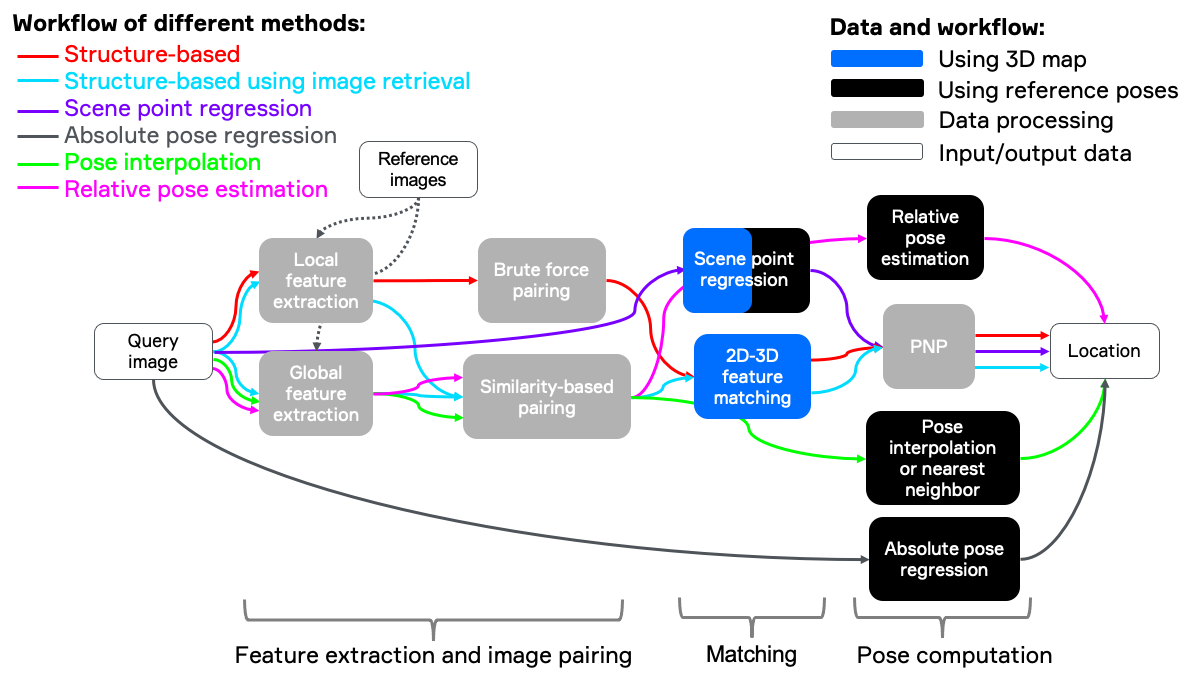
\includegraphics[width=\textwidth]{pics/Chapter2/overviewViLoc.png}
    \caption{Tổng quát về những phương pháp định vị trực quan quan trọng \cite{methodsLocal}}
\end{figure}

\subsection{Những phương pháp sử dụng biểu diễn 3D}
\subsubsection*{Ý tưởng}
Những phương pháp sử dụng biểu diễn 3D sẽ hoạt động xoay quanh việc tái tạo lại môi trường đang xét bằng một bản đồ đám mây điểm 3D. Bản đồ 3D chứa những đặc trưng trích xuất được từ các ảnh và tiến hành kiếm các cặp đặc trưng tương quan giữa các ảnh với nhau nhằm tạo thành những điểm mô tả 3D trong không gian ba chiều. Những bản đồ này thường sẽ được mô hình tạo ra vào lúc tiền xử lý tập dữ liệu và sẽ được dùng trong suốt quá trình bản địa hóa của mô hình.
\subsubsection*{Những bước thực hiện}
\begin{itemize}
    \item Ở bước tiền xử lý, không gian được thể hiện bởi tập dữ liệu sẽ được tái tạo lại trong không gian 3D, sử dụng những ảnh cùng thể hiện một cảnh, nhưng từ những vị trí và góc nhìn khác nhau. Phương pháp tái tạo này được gọi là Tái tạo kiến trúc từ chuyển động - Structure from Motion. Cụ thể hơn, quá trình này sẽ gồm các giai đoạn:
          \begin{itemize}
              \item Trích xuất mô tả của các đặc trưng từ ảnh: Mỗi ảnh trong tập dữ liệu sẽ được trích xuất đặc trưng và mỗi đặc trưng sẽ được gán một giá trị mô tả để SfM có thể tìm được những đặc trưng tương đồng giữa các hình. Kết quả đầu ra sẽ là một tập các mô tả cho đặc trưng của từng ảnh.
              \item Tìm kiếm sự tương quan của các đặc trưng giữa các ảnh: SfM sẽ tìm kiếm những ảnh cùng nhìn bộ phận của cảnh bằng cách kiểm tra sự tương đồng giữa các mô tả của đặc trưng trên các ảnh. Những cặp ảnh chứa những cặp đặc trưng tương quan sẽ cần được xác nhận lại về tính đúng đắn về hình học qua việc có tồn tại một cách biến đổi có khả năng ánh xạ một số lượng trưng giữa hai ảnh.
              \item Tái tạo lại cấu trúc: Quá trình tái tạo lại cấu trúc sẽ bắt đầu từ một cặp ảnh khởi tạo. Sau đó, không gian điểm 3D sẽ dần được mở rộng khi các ảnh được thêm tuần tự qua giải thuật PnP trong vòng lặp RANSAC.
          \end{itemize}
    \item Sau khi có được bản đồ đám mây điểm 3D biểu diễn môi trường đang xét, khi mô hình nhận vào một ảnh mới, những đặc trưng trong ảnh sẽ được trích xuất và so sánh mô tả của chúng với những điểm trong bản đồ 3D của khu vực. Khi những cặp đặc trưng 2D-3D đã được xác định, giải thuật PnP trong vòng lặp RANSAC sẽ được sử dụng một lần nữa để xác định vị trí của ảnh được chụp.
\end{itemize}
\subsubsection*{Những biến thể của phương pháp}

Một trong những tác vụ quan trọng nhất trong bài toán định vị bằng biểu diễn 3D chính là việc trích xuất ra được đặc trưng của ảnh và tạo cách mô tả thích hợp cho chúng. Ở những phương pháp truyền thống, những giải thuật được định nghĩa thủ công như SIFT \cite{lowe2004distinctive} và SURF \cite{bay2006surf} sẽ được sử dụng. Tuy nhiên, ở những giải thuật này tồn tại một số điểm yếu, xuất phát từ việc chúng không được thiết kế đặc biệt cho tác vụ hiện tại là truy xuất những ảnh biểu diễn cảnh giống nhau. Điều này sẽ làm giảm hiệu quả, đặc biệt trong điều kiện thay đổi như ngày-đêm, thay đổi theo mùa. Trong khoảng thời gian gần đây, những hướng tiếp cận theo hướng học sâu đã được đề xuất, chủ yếu sử dụng mạng CNN để trích xuất và biểu diễn đặc trưng. Những cách tiếp cận này vẫn gặp khó khăn trong việc nhận biết được những đặc điểm hình học trong hình \cite{zhou2020learn}.

Để có thể biểu diễn chính xác được một thành phố lớn trong không gian 3D, một lượng lớn điểm 3D sẽ cần được sử dụng. Với tập dữ liệu Aachen Day-Night \cite{sattler2018benchmarking}, mô hình 3D sẽ có số lượng điểm dao động từ 700 nghìn cho đến 2.5 triệu, tùy thuộc vào số lượng cặp ảnh được dùng. Vì vậy, chiến lược tìm kiếm Brute-Force sẽ dần trở nên bất khả thi khi môi trường biểu diễn trở nên lớn hơn. Để giới hạn lại không gian tìm kiếm, chiến lược truy xuất ảnh đã được sử dụng để tìm kiếm ảnh trong tập dữ liệu tương đồng nhất với ảnh truy vấn. Sau đó, việc tìm kiếm tương quan sẽ chỉ diễn ra trong không gian được thể hiện bởi những ảnh đó \cite{sarlin2019coarse}.

Để không phải lưu trữ một bản đồ 3D cho toàn khu vực đang xét, một phương pháp khác đã được đề xuất là xây dựng bản đồ điểm 3D cục bộ. Thay vì sinh ra bản đồ 3D cho toàn bộ khu vực đang xét ở bước tiền xử lý, phương pháp này sẽ sử dụng những ảnh truy xuất được để sinh ra bản đồ cục bộ \cite{sattler2017large}. Phương pháp này có thể tận dụng được những điểm mạnh của việc sử dụng cách biểu diễn 3D mà không cần duy trì bản đồ điểm 3D của toàn bộ khu vực. Tuy nhiên, cách tiếp cận này vẫn có một số điểm yếu như việc thời gian chạy trở nên đáng kể và số lượng ảnh truy xuất được có thể chưa đủ để sinh ra một bản đồ 3D phù hợp.

Một cách tiếp cận khác với mục tiêu loại bỏ sự cần thiết của bản đồ 3D, sử dụng mạng học sâu để xác định được vị trí của một điểm ảnh trong môi trường 3D, gọi là hồi quy điểm trong cảnh - Scene Point Regression \cite{brachmann2021visual}. Tuy nhiên, những mô hình thuộc phương pháp này không có tính khái quát hóa mà để có thể chạy trên một khu vực nhất định thì mô hình cần dữ liệu mẫu thuộc khu vực đó để huấn luyện.
\newpage
\subsubsection*{Phân tích ưu và nhược điểm của phương pháp}
Nhờ vào việc sử dụng cách biểu diễn trong không gian 3D, lớp phương pháp này đã thành công học được tính hình học của môi trường, nhờ vậy nên những kết quả của lớp phương pháp này thường sẽ đạt được kết quả định vị chính xác. Ngoài ra, lớp phương pháp này sử dụng điểm 3D trong không gian làm mốc để định vị. Nhờ vậy nên mô hình vẫn sẽ cho ra được kết quả tốt khi không gian mẫu của vị trí chụp của ảnh bị giới hạn.

\begin{figure}[H]
    \centering
    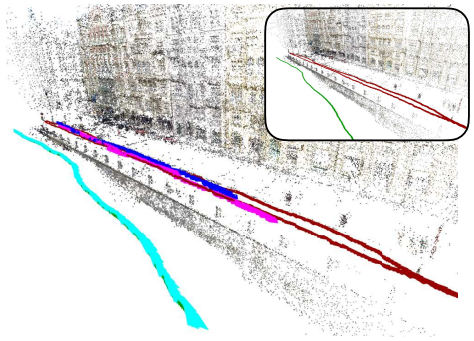
\includegraphics[scale=0.7]{pics/Chapter2/lim.png}
    \caption[Kịch bản so sánh phương pháp 3D và phương pháp sử dụng biểu diễn ngầm \cite{sattler2019understanding}]{Kịch bản khi mà tập dữ liệu huấn luyện bị hạn chế. Quỹ đạo của tập huấn luyện và tập kiểm thử có màu \textcolor{red}{đỏ} và \textcolor{green}{xanh lá}. Kết quả của những mô hình lấy vị trí của ảnh làm mốc là PoseNet \cite{kendall2016posenet} và MapNet \cite{brahmbhatt2018geometryaware} có quỹ đạo kết quả màu \textcolor{blue}{xanh dương} và \textcolor{purple}{tím}. Kết quả của phương pháp sử dụng biểu diễn 3D là Active Search \cite{sattler2016efficient} có quỹ đạo màu \textcolor{cyan}{xanh lam}}
\end{figure}

Đa số những vấn đề xoay quanh lớp phương pháp này sẽ liên quan đến việc sinh ra, lưu trữ và sử dụng biểu diễn 3D của khu vực. Do những bản đồ 3D biểu diễn những khu vực lớn sẽ có nhiều điểm 3D, dẫn đến việc tiêu tốn nhiều tài nguyên tính toán để sinh ra và sử dụng, đồng thời cần nhiều bộ nhớ để lưu trữ. Ngoài ra, đánh đổi cho khả năng biểu diễn một khu vực với độ chi tiết cao, những mô hình sử dụng cách biểu diễn 3D sẽ mất khả năng khái quát hóa khi xử lý những ảnh bên ngoài khu vực đang xét và cần phải được huấn luyện lại trên tập dữ liệu khác.

\subsection{Những phương pháp hồi quy vị trí}
\subsubsection*{Ý tưởng}
Với những thành công gần đây trong các tác vụ của ngành khoa học máy tính như phân loại ảnh, phân vùng ảnh theo ngữ nghĩa, truy xuất ảnh, những phương pháp sử dụng mạng học sâu đã có thể phần nào trích xuất được những thông tin hình học từ ảnh. Sử dụng những thông tin này, mô hình học sâu có thể xây dựng một hàm ánh xạ đến những cách biểu diễn mong muốn. Vì tính linh hoạt của hướng tiếp cận học sâu nên chúng có thể được ứng dụng để thay thế một hay nhiều tác vụ bên trong quá trình giải bài toàn định vị trực quan.

\newpage
\subsubsection*{Những bước thực hiện}

Để những phương pháp học sâu có thể hoạt động một cách hiệu quả, mô hình cần được cung cấp một tập dữ liệu đã có kết quả để huấn luyện trên đó. Sau đó, mô hình học sâu có thể biến đổi dữ liệu đầu vào thành kết quả một cách trực tiếp, không cần sự can thiệp của con người. Cụ thể hơn, một phương pháp hồi quy vị trí sẽ thường có những bước sau:
\begin{itemize}
    \item Huấn luyện mô hình trên tập dữ liệu mẫu: Mô hình sẽ được huấn luyện qua tập dữ liệu mẫu để có thể chọn được những chi tiết chứa thông tin quan trọng để trích xuất. Quá trình này có thể được tăng tốc và cải thiện độ chính xác bằng cách sử dụng hàm mất mát và cấu trúc mô hình phù hợp với bài toán, cũng như tích hợp thêm thông tin từ cảm biến.
    \item Thực thi mô hình
          \begin{itemize}
              \item Mã hóa dữ liệu: Đầu tiên, khi đầu vào là một ảnh, những lớp CNN của mô hình sẽ tiến hành trích xuất những chi tiết có thông tin bên trong hình, tiến hành mã hóa hình thành một tập các giá trị đại diện. Trong những năm gần đây, hướng tiếp cận sử dụng Vision Transformer đã đem lại hiệu quả hơn so với những mô hình CNN thông thường.
              \item Ánh xạ tới cách biểu diễn phù hợp: Những giá trị mã hóa của một ảnh có thể được dùng để ánh xạ trực tiếp ra những cách biểu diễn đã được định nghĩa từ trước.
          \end{itemize}
\end{itemize}
\subsubsection*{Những biến thể của phương pháp}

Hồi quy vị trí tuyệt đối là một nhóm phương pháp mà mô hình học sâu sẽ được dùng để trực tiếp tính toán ra vị trí của ảnh. PoseNet \cite{kendall2016posenet} là một phương pháp đặc trưng của hướng tiếp cận này. Những mô hình CNN cơ sở như VGGNet hoặc ResNet sẽ được loại bỏ lớp Softmax cuối cùng và được thay thế bằng những lớp kết nối đầy đủ để xác định được vị trí và góc quay của ảnh. Một số cải thiện đã được đề xuất cho mô hình này như việc giới thiệu một hàm mất mát mới, áp dụng những lớp mạng trích xuất tốt hơn(LSTM, Vision Transformer,\dots) \cite{keetha2023anyloc} hoặc tích hợp thêm dữ liệu từ cảm biến như ngữ nghĩa của cảnh, độ sâu của cảnh \cite{yan2022crossloc}, hướng quay của vật bên trong hình \cite{liu2019lending} \dots

Nhóm phương pháp tiếp theo không xác định vị trí chụp ảnh một cách trực tiếp, mà nhờ vào việc tìm được độ lệch giữa ảnh truy vấn với một ảnh tham khảo đã biết trước vị trí và góc quay. Các bước thực hiện bao gồm hai bước là nhận dạng địa điểm trực quan nhằm truy xuất ảnh tham khảo, và hồi quy vị trí tương đối nhằm xác định được độ lệch vị trí và góc quay giữa cặp ảnh. Phương pháp này sẽ được cải thiện khi áp dụng những mô hình cơ sở có khả năng trích xuất tốt hơn \cite{shavit2023coarse}. Ngoài ra, nếu như những thông số của máy ảnh được cung cấp, độ lệch về vị trí và góc quay của cặp ảnh có thể được xác định từ việc tìm kiếm cặp đặc trưng tương quan giữa hai hình từ ma trận thiết yếu \cite{zhou2020learn}.

\subsubsection*{Phân tích ưu và nhược điểm của phương pháp}
Việc ứng dụng mô hình học sâu vào bài toán này sẽ loại bỏ được như cầu xử lý dữ liệu bằng tay. Những mạng nơ-ron sẽ có thể khám phá được những cách trích xuất hiệu quả hơn, hoạt động tốt hơn trong những điều kiện thay đổi như ngày-đêm, các mùa trong năm. Ngoài ra, quá trình xử lý dữ liệu của nhóm phương pháp này sẽ yêu cầu ít hơn về tài nguyên và có thời gian chạy ngắn do chỉ cần chạy qua mô hình một lần. Cuối cùng, phương pháp này có thể tận dụng được những mô hình cơ sở CNN đã cho ra kết quả tốt trong những tác vụ thị giác máy tính khác.

Tuy nhiên, việc ứng dụng những mô hình học sâu cũng có một số điểm yếu. Đa số các mô hình hồi quy hiện tại chỉ thí nghiệm trên những tập dữ liệu trong phạm vi nhỏ và có sự phân bố dày đặc. Ngoài ra, độ chính xác của những phương pháp hồi quy cũng sẽ không thể bằng được so với phương pháp sử dụng biểu diễn 3D do những mô hình CNN cơ sở vẫn còn gặp khó khăn trong việc học được những thông tin hình học \cite{zhou2020learn}. Đối với những mô hình hồi quy vị trí tuyệt đối, môi trường đang xét sẽ được biểu diễn ngầm trong những trọng số của mô hình, làm mất đi khả năng khái quát hóa tới khu vực khác của mô hình \cite{sattler2019understanding}. Còn với những mô hình sử dụng hồi quy vị trí tương đối, hiệu quả sẽ bị ảnh hưởng lớn bởi quá trình truy xuất ảnh ban đầu.

\subsection{Kết luận}
Trong những lớp phương pháp giải quyết bài toán định vị trực quan, hướng tiếp cận sử dụng cách biểu diễn 3D có kết quả vượt trội hơn hẳn. Tuy nhiên, để đánh đổi cho độ chính xác này, nhóm phương pháp này đã mất đi tính khái quát hóa cho những tập dữ liệu khác, cũng như tiêu tốn một lượng tài nguyên lớn để khởi tạo và duy trì bản đồ 3D. Hướng tiếp cận hồi quy vị trí tuyệt đối cũng gặp phải vấn đề về khả năng khái quát cùng với độ chính xác chưa tốt.

Nhằm hướng đến một giải pháp có khả năng khởi tạo/huấn luyện một lần mà có thể chạy được trên nhiều môi trường khác nhau, chúng tôi đã chọn phát triển phương pháp theo hướng kết hợp nhận dạng địa điểm trực quan và hồi quy vị trí tương đối nhằm cho ra kết quả cạnh tranh mà không tiêu tốn quá nhiều tài nguyên, cả bộ nhớ và năng lực tính toán.

Một giải pháp hoàn chỉnh sẽ bao gồm hai thành phần là \textbf{truy xuất ảnh} và \textbf{hồi quy tương đối}. Ở những phần sau, những giải pháp đã được đề xuất trong hai lĩnh vực này sẽ được khảo sát.


\section{Nhận dạng địa điểm trực quan - Visual Place Recognition}

Để đáp ứng nhu cầu xác định vị trí của ảnh với độ chính xác trên 6 bậc tự do (6 Degrees of Freedom), việc thu thập thông tin 3 chiều của bối cảnh bằng cảm biến LiDAR, hoặc chế tạo mô hình 3 chiều của bối cảnh bằng các hướng tiếp cận mô hình từ chuyển động (Structure from Motion) để ước tính tư thế của máy ảnh ngày càng được các nhà nghiên cứu sử dụng vì tính chính xác cao và độ bền tốt trước các yếu tố thay đổi về môi trường như ánh sáng và các bề mặt phản chiếu, ... Tuy tận dụng được lợi thế về tính phổ biến ngày càng cao của các phương tiện tự động lái với cảm biến độ sâu và cảm biến LiDAR, các hướng tiếp cận này đều có chi phí và yêu cầu tài nguyên rất lớn để duy trì và phát triển, giới hạn quy mô giải pháp về  cả không gian và thời gian. Vấn đề này bắt nguồn từ yêu cầu thu thập, lưu trữ và cập nhật dữ liệu đám mây điểm. Vì lý do này, một nhánh phát triển của bài toán định vị trực quan trên quy mô lớn (large-scale visual localization) tìm cách giải quyết bài toán từ góc nhìn của bài toán truy xuất hình ảnh\cite{2022arXiv220105816X} (Image retrieval/Instance retrieval).

Bằng cách sử dụng một cơ sở dữ liệu hình ảnh đã được gắn nhãn với thông tin tư thế và vị trí, việc duy trì mô hình dự đoán trở thành việc duy trì cơ sở dữ liệu ảnh RGB(3 kênh màu đỏ - xanh lá - xanh dương) 2 chiều được gắn nhãn. Điều chỉnh các phương pháp truy xuất hình ảnh hiện có để phù hợp hơn với bài toán định vị, với một ảnh truy vấn (query image), mục tiêu định vị trực quan lúc này trở thành việc xác định hình ảnh tương tự nhất với ảnh truy vấn trong cơ sở dữ liệu chứa các ảnh đã được gắn nhãn với thông tin định vị, từ đó, tính toán tư thế thật của ảnh truy vấn. Sử dụng phương pháp này, bài toán định vị trực quan có thể được chia thành hai bước: truy xuất hình ảnh trực quan (Visual Place Recognition) và ước tính tư thế máy ảnh từ hình ảnh truy xuất được (Pose Estimation). Trong đó, bước truy xuất hình ảnh trực quan thường được hiện thực thành quy trình ba bước\cite{Masone2021ASO}:

\begin{enumerate}
    \item bước trích xuất và mã hóa đặc trưng trích xuất một véc-tơ biểu diễn từ mỗi ảnh trong cơ sở dữ liệu để đại diện cho nội dung của ảnh (\textit{image representation});
    \item bước tìm kiếm tương đồng sử dụng các thuật toán so sánh tương đồng để đánh giá và tìm các ảnh trong cơ sở dữ liệu có nội dung tương tự nhất với ảnh truy vấn;
    \item bước hậu xử lý để lọc, sắp xếp và tinh chỉnh kết quả trả về từ bước tìm kiếm tương đồng, đưa ra kết quả cuối cùng.
\end{enumerate}

Sử dụng và duy trì cơ sở dữ liệu ảnh RGB 2D làm giảm đáng kể chi phí duy trì, cũng như chi phí cập nhật và thu thập dữ liệu so với dữ liệu đám mây điểm, cho phép triển khai các mô hình truy xuất nhỏ và nhẹ với tốc độ truy xuất cao. Tuy nhiên, việc phụ thuộc vào dữ liệu có được từ cảm biến RGB máy ảnh thông dụng đặt mô hình trước các thách thức mà các phương pháp truy xuất bằng dữ liệu 3 chiều đã tránh khỏi dẫn đến hiệu năng thấp hơn. Ở đề mục này, chúng tôi sẽ trình bày quá trình phát triển, các giải pháp nền tảng và các hướng tiếp cận hiện đại để giải quyết các vấn đề nêu trên, tăng hiệu năng truy xuất và mức độ thông tin hiệu dụng có thể truyền cho bước định vị tư thế.

\subsection{Trích xuất và biểu diễn đặc trưng}

Dưới góc nhìn một bài toán truy xuất ảnh, các đặc trưng biểu diễn của ảnh sẽ mang tính quyết định đối với chất lượng và hiệu năng của cả mô hình. Để đảm bảo khả năng biểu diễn tốt cho các đặc trưng ảnh ở các địa danh khác nhau, quá trình trích xuất đặc trưng, ban đầu, được thiết kế một cách thủ công, đến từ kiến thức chuyên môn. Các nghiên cứu bước đầu đặt ra các định nghĩa về các loại đặc trưng: đặc trưng lân cận, đặc trưng toàn cục và độ quan trọng của chúng. Thời gian gần đây, với sự phát triển của thị giác máy tính, các phương pháp học biểu diễn bằng mạng neuron học sâu đạt được các thành tựu nổi bật, đặc biệt là mạng neuron tích chập thay thế chức năng của đặc trưng thủ công.

\subsubsection{Biễu diễn đặc trưng lân cận - Local descriptors}

Trong bài toán học biễu diễn đặc trưng, một đặc trưng lân cận chỉ phân tích, biểu diễn ý nghĩa của một nhóm các điểm ảnh nhỏ và chỉ ra sự khác biệt giữa chúng với các nhóm các điểm ảnh lân cận \cite{CGV-017-localdescriptors}. Các nhóm điểm ảnh được tạo ra bằng cách chia mỗi hình ảnh thành lưới với độ phân giải nhất định và tất cả các nhóm điểm ảnh được thu thập, trích xuất để tìm đặc trưng. Để áp dụng cho bài toán truy xuất hình ảnh trực quan, các thuật toán lựa chọn như Hessian-Affine detector \cite{hessian-affine-detector}, MSER\cite{MSER-detector} được áp dụng để lựa chọn chỉ những nhóm điểm ảnh mang tính quan trọng, quyết định đến sự khác nhau giữa các ảnh và loại bỏ các nhóm điểm ảnh dễ bị ảnh hưởng bởi yếu tố môi trường. Vào thời gian đầu, việc truy xuất đặc trưng từ các nhóm ảnh, điểm ảnh được thực hiện bằng cách sử dụng các thuật toán như SIFT \cite{lowe1999object}, SURF \cite{bay2006surf}, RootSIFT \cite{Arandjelovi2012ThreeTE}, BRIEF \cite{brief}, DSP-SIFT \cite{Dong2014DomainsizePI} và đặc trưng kernel \cite{kernel-descriptors}. Các hướng tiếp cận mới hơn cho rằng các hướng tiếp cận trên sử dụng số lượng lớn đặc trưng cần trích xuất và lưu trữ trong khi không phải tất cả các đặc trưng đều có đủ tính phân biệt cho quá trình truy xuất ảnh \cite{predicting-good-features}, từ đó, đề xuất thêm quá trình lọc đặc trưng vào quá trình trích xuất. Năm 2014, Jégou và Zisserman chuẩn hóa quá trình trích xuất vector biểu diễn từ đặc trưng cục bộ thành quy trình 2 bước\cite{Jegou_2014_CVPR}:
\begin{enumerate}
    \item bước nhúng chuyển mỗi vector đặc trưng lên không gian mới có số chiều cao hơn,
    \item bước tổng hợp tạo chỉ một vector biểu diễn từ các vector đã tạo.
\end{enumerate}
Năm 2015, \cite{selective-match-kernel} đề xuất hàng loạt các phương án cho các bước nhúng, tổng hợp, cùng với các giải pháp để lựa chọn mức độ đóng góp của mỗi cặp biểu diễn cho một nhóm các ảnh, đánh dấu nền móng về hướng phát triển và hiện thực cho các mô hình học biễu diễn đặc trưng cục bộ sau này.

\subsubsection{Biễu diễn đặc trưng toàn cục  - Global descriptors}

Trong khi việc tổng hợp các vector biểu diễn cục bộ hỗ trợ việc truy xuất một vector biễu diễn cho một hình ảnh, các vector biểu diễn toàn cục có thể truy xuất tất cả thông tin này một cách trực tiếp. Khác với vector trích xuất cục bộ, các vector trích xuất toàn cục đọc và trích xuất biểu diễn đặc trưng cho toàn bộ bức ảnh và chỉ ra các đặc điểm khác biệt giữa bức ảnh này và bức ảnh khác. Việc truy xuất vector toàn cục có thể được hiện thực và thực thi với yêu cầu tài nguyên ít hơn sơ với việc truy xuất vector cục bộ, nhưng đồng thời cũng giảm đi khả năng phân biệt và tính bền bỉ trước các yếu tố thay đổi do điều kiện môi trường, góc chụp và các yếu tố bị che khuất. Mặc dù vậy, lợi ích của việc trích xuất đặc trưng cục bộ, áp dụng bởi các phương pháp như HOG \cite{HOG}, Gist \cite{GIST}, vẫn được xem trọng trong quá trình trích xuất biểu diễn đặc trưng toàn cục và trở thành cảm hứng cho các mô hình học biểu diễn sử dụng mạng neuron học sâu sau này.

\subsubsection{Học biễu diễn bằng mạng neuron học sâu tích chập và các lớp kết nối đầy đủ}

Với sự thành công của mạng neuron học sâu trong lĩnh vực thị giác máy tính\cite{krizhevsky2012imagenet}, các mô hình học sâu này đã được công nhận là những phương pháp tạo biểu diễn vô cùng hiệu quả. Đồng thời, một số bài báo cũng đã chỉ ra khả năng học đặc trưng thường thấy và chuyển tiếp được (transferable) đến các bài toán khác \cite{Oquab_2014_CVPR,ZeilerVisualizingAU,Chen2018DeepLabSI}.

\begin{figure}[h]
    \centering
    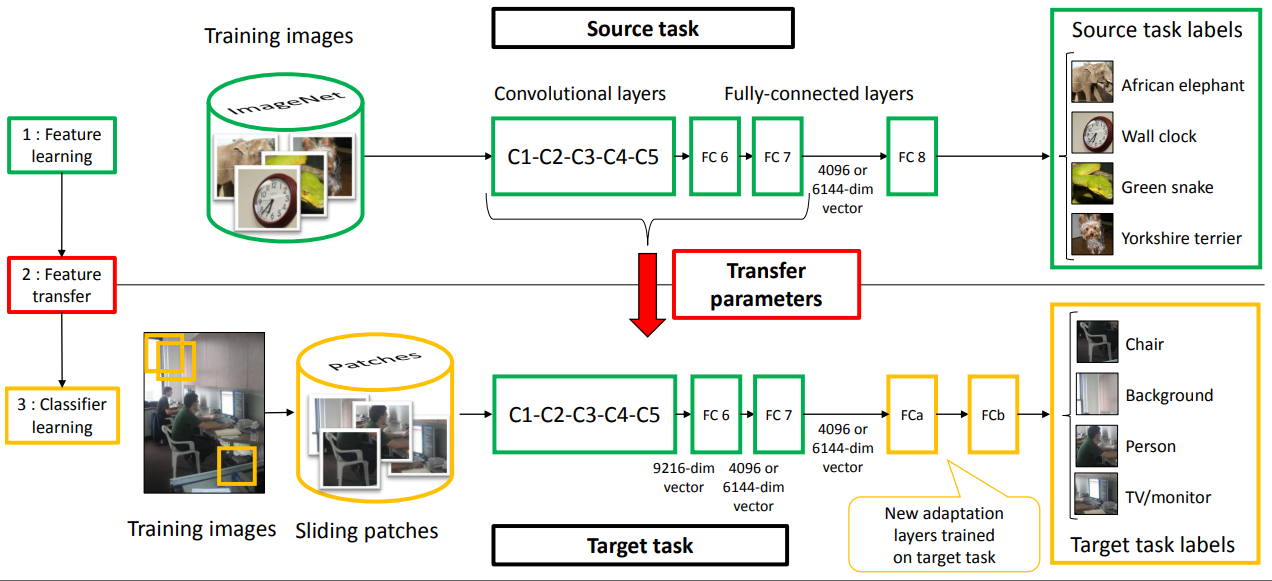
\includegraphics[width=\textwidth]{pics/Chapter2/cnn_transfer.png}
    \caption{Chuyển tiếp thông số của một mô hình mạng neuron học sâu tích chập\cite{Oquab_2014_CVPR}}
\end{figure}

Các mô hình học sâu tích chập đầu tiên được sử dụng cho bài toán truy xuất hình ảnh trực quan được cấu hình từ các lớp kết nối đầy đủ\cite{razavian2014cnn, gong2014multiscale, babenko2014neural, deepindex, image-classification-retrieval, wang2014deep} của một mạng phân loại, được huấn luyện trên tập dữ liệu ImageNet\cite{russakovsky2015imagenet}, đạt hiệu quả đáng kể khi sử dụng hàm mất mát triplet\cite{wang2014deep, gomezojeda2015training}. Tuy nhiên, có thể sớm nhận thấy rằng các mô hình sử dụng nhiều lớp kết nối đầy đủ có ý nghĩa tương ứng với các biểu diễn đặc trưng toàn cục. Các biểu diễn đặc trưng tạo ra được bằng cách sử dụng phương pháp này thiếu độ bền đối với dữ liệu chứa nhiều yếu tố gây nhiễu, che khuất và không đủ các yếu tố bất biến đối với biến thể tịnh tiến và tỉ lệ. Để khắc phục các hạn chế này, nhiều mô hình học sâu đã đề xuất các phương án cắt ảnh thành nhiều nhóm điểm ảnh và huấn luyện nhiều biểu diễn với kết nối đầy đủ cho mỗi hình \cite{razavian2014cnn, babenko2014neural}. Khi đánh giá các cách tiếp cận này so với các phương pháp trích xuất đặc trưng thủ công cục bộ, các mô hình học sâu sử dụng ít bộ nhớ hơn nhưng yêu cầu số lượng tính toán cao hơn. Các biểu diễn kết nối đầy đủ bị giới hạn bởi kích thước đầu vào cố định và lượng lớn các tham số.

\subsubsection{Học biểu diễn bằng mạng neuron tích chập}

Nỗ lực tìm giải pháp cho các giới hạn của mạng neuron kết nối đầy đủ đã trở thành cảm hứng cho các phương pháp sử dụng trực tiếp kết quả nhận được từ các lớp tích chập của mạng neuron học sâu. Áp dụng hướng tiếp cận đầu tiên chính là bài nghiên cứu của Babenko và nnk \cite{babenko2014neural}. Mạng neuron tích chập tạo ra một tenxơ (tensor) có cấu hình \(H \times W \times C\), trong đó \(C\) là số kênh, \(H\) và \(W\) là chiều cao và chiều rộng của ảnh. Babenko và nnk tạo ra vector biểu diễn bằng cách làm phẳng và chuẩn hóa lớp \(H \times W \times C\). Một số bài báo lấy cảm hứng từ hướng nghiên cứu này \cite{hou2015convolutional}, sau đó, đã thể hiện rằng vector biểu diễn mạng neuron học được, tùy vào phương án kết hợp lớp tenxơ, có thể mang ý nghĩa và chức năng tương tự với biểu diễn đặc trưng toàn cục trong khi tránh được các hạn chế của các mô hình học sâu sử dụng lớp kết nối đầy đủ. Các giải pháp này có thể được phân loại vào hai nhóm chính \cite{Masone2021ASO}:

\begin{itemize}
    \item gom cụm đặc trưng (feature aggregation) tích chập bằng các giải pháp lấy cảm hứng từ trích xuất đặc trưng thủ công cục bộ;
    \item tổng hợp đặc trưng (feature pooling) bằng cách khái quát hóa các đặc trưng tích chập.
\end{itemize}

\begin{figure}[h]
    \centering
    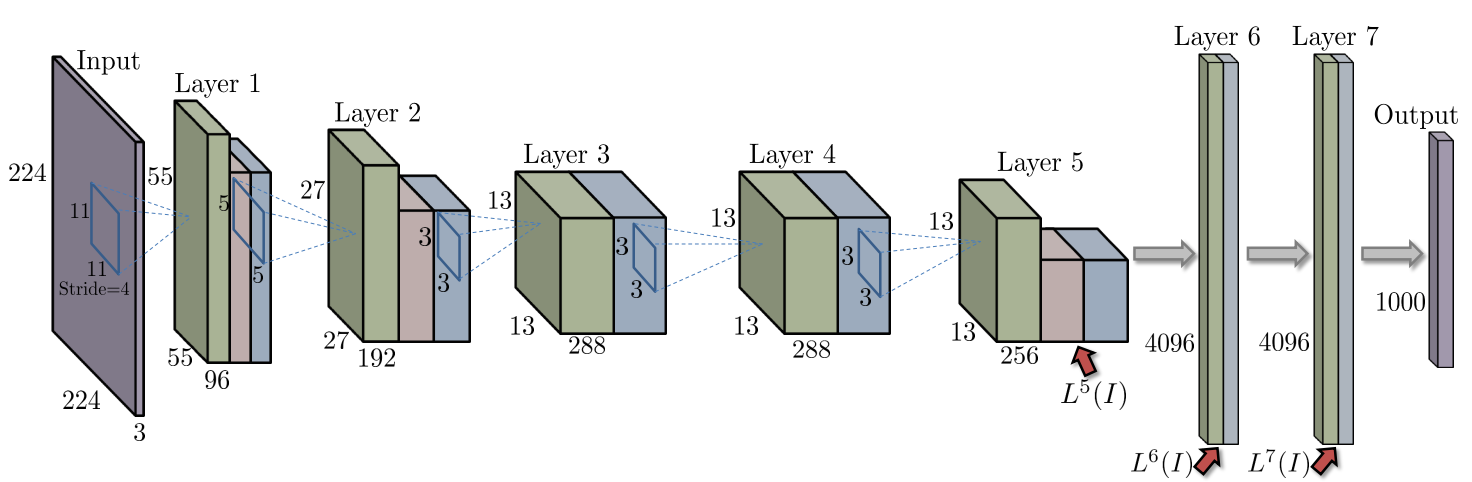
\includegraphics[width=\textwidth]{pics/Chapter2/firstcnns.png}
    \caption{Minh họa kiến trúc một mô hình CNN \cite{babenko2014neural}}
\end{figure}

Khi thực hiện gom đặc trưng trên lớp đặc trưng \(H \times W \times C\), lớp tích chập được đặt dưới góc nhìn là một lưới \(H \times W \) chứa các đặc trưng \(C\) chiều với mỗi đặc trưng là một vector có vùng nhận thức nhỏ. Bằng cách này, kết quả nhận được từ lớp tích chập có thể được đồng hóa (assimilated) thành một tập hợp các vector cục bộ được bố trí dày đặc. Tập hợp các vector dày đặc tiếp tục được mã hóa thành một vector biểu diễn và được sử dụng cho quá trình so sánh và truy xuất bằng các giải thuật so sánh tương đồng như khoảng cách Euclidean, tương đồng cosine. Sử dụng phương pháp này, việc mã hóa đặc trưng cho bước tìm kiếm tương đồng có thể áp dụng các hướng tiếp cận xử lý đặc trưng thủ công cục bộ như VLAD\cite{vlad}, BoW\cite{Mohedano_2016}, ASMK\cite{cao2020unifying}. Các nhà nghiên cứu tiếp tục đề xuất các phương pháp gom cụm có khả năng kết hợp trực tiếp với mạng neuron tích chập toàn bộ để cung cấp khả năng huấn luyện cả mô hình đầu-cuối \cite{ong2017siamese}. Đánh dấu một bước tiến quan trọng trong nỗ lực tìm giải pháp cho bài toán nhận diện địa điểm trực quan chính là lớp gom cụm NetVLAD \cite{arandjelovic2016netvlad}, hiện thực mô hình mã hóa và gom cụm VLAD với các phép tính khả vi cho phép mô hình khả năng huấn luyện đầu cuối một cách linh hoạt với nhiều tham số huấn luyện hơn so với VLAD thông thường. Hướng tiếp cận của các tác giả NetVLAD được tiếp tục hiện thực và sử dụng đến nay, đồng thời trở thành cảm hứng cho các hướng tiếp cận hiện đại hơn sau này.

\begin{figure}[h]
    \centering
    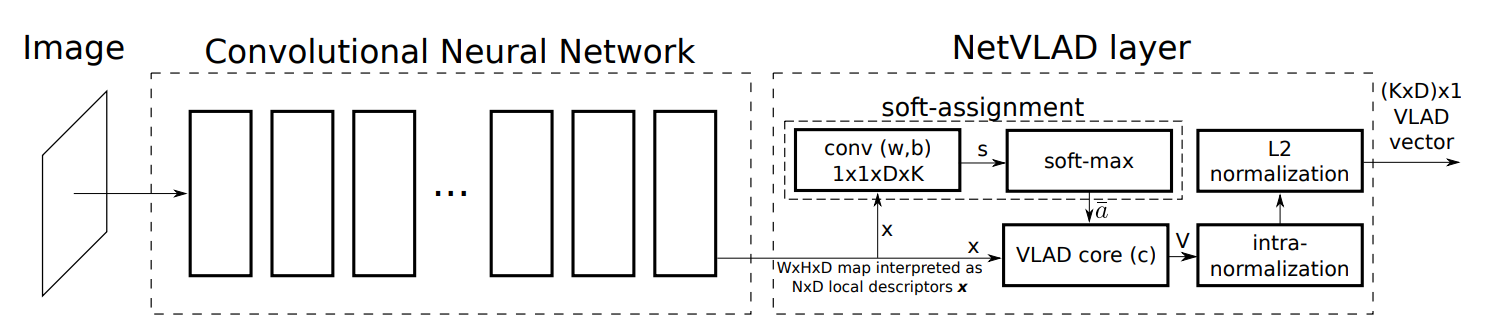
\includegraphics[width=\textwidth]{pics/Chapter2/netvladcnn.png}
    \caption{Minh họa kiến trúc một mô hình CNN được kết nối với lớp NetVLAD \cite{arandjelovic2016netvlad}}
\end{figure}

Tổng hợp đặc trưng lấy cảm hứng từ các nghiên cứu về mạng neuron tích chập. Các nhà nghiên cứu đã chỉ ra các đặc trưng từ những lớp tích chập giữa, cuối có tiềm năng được gom đặc trưng và sử dụng trực tiếp cho quá trình phân loại và tìm kiếm tương qua mà không cần mã hóa. Quá trình tổng hợp đặc trưng, tuy có thể được thực hiện một cách tương đối đơn giản như việc sử dụng một lớp max-pooling, lại truy xuất được các đặc trưng biểu diễn với số chiều thấp, mức chiếm dụng bộ nhớ thấp và hiệu năng vượt trội hơn so với đặc trưng biểu diễn được thiết kế thủ công. Các tác giả của bài báo \cite{mousavian2015deep} nhận thấy rằng phương pháp max-pooling có độ bền cao hơn đối với sự thay đổi về tỉ lệ trong khi sum-pooling có độ nhạy với các yếu tố gây nhiễu hơn. Họ kiểm thử một mô hình kết hợp cả hai phương pháp, SPoC, với mục đích đúc kết được điểm mạnh của cả hai phương pháp và đã đạt kết quả đáng kể. Tương tự, Tolias và những cộng sự \cite{tolias2015particular} phát triển quy trình mã hóa R-MAC (Regional Maximum Activations of Convolutions), tính toán vector max-pooling cho nhiều vùng ảnh khác nhau và tổng hợp chúng bằng lớp sum-pooling. R-MAC và SPoC là cảm hứng cho sự ra đời của GeM \cite{GeM} - lớp aggregation trung bình tổng quát. Áp dụng một tham số cho mỗi lớp đặc trưng và hiện thực lớp trung bình tổng quát dự trên các tham số đó, GeM đạt được hiệu quả vượt trội hơn cả R-MAC và SPoC và trở thành một trong những phương pháp tổng hợp đặc trưng hiệu quả nhất cho đến nay.

\subsection{Học nhận diện địa điểm trực quan}

Để đạt hiệu quả cao trong bài toán nhận diện địa điểm trực quan, ngoài việc truy xuất được các biểu diễn đặc trưng tốt, nhiều nghiên cứu còn tập trung phát triển quá trình học truy xuất, đặt quá trình huấn luyện mô hình dưới nhiều hướng tiếp cận khác nhau. Các hướng tiếp cận này có thể được chia thành hai nhóm chính: học truy xuất thông qua phân loại và học để xếp hạng. Ngoài ra, một số nghiên cứu còn tập trung vào khả năng học từ kiến thức chuyên môn hoặc tối ưu hóa quá trình học để xếp hạng với hàm mất mát lấy cảm hứng từ phương pháp xếp hạng danh sách (listwise ranking).

\subsubsection{Học truy xuất thông qua phân loại}

Vì bài toán phân loại là một trong những bài toán đầu tiên thể hiện kết quả tốt khi áp dụng mạng nơ-ron tích chập vào quá trình trích xuất đặc trưng, các mô hình học sâu tích chập được sử dụng cho bài toán nhận diện địa điểm trực quan đầu tiên lấy cảm hứng lớn từ các mô hình phân loại thay vì các mô hình truy xuất. Các mô hình này sử dụng một mạng nơ-ron tích chập đã được huấn luyện trên tập dữ liệu ImageNet \cite{krizhevsky2012imagenet}. Học truy xuất thông qua phân loại cho phép các nhà nghiên cứu huấn luyện được các véc-tơ đặc trưng toàn cục với kích thước nhỏ, sử dụng nhãn ở cấp độ ảnh mà không cần khai phá thông tin tương quan (example mining) trong quá trình huấn luyện, dẫn tới yêu cầu tài nguyên tính toán thấp hơn đáng kể so với các mô hình hiện tại, có tiềm năng lớn trong việc mở rộng phạm vi của bài toán truy xuất lên các tập dữ liệu lớn. Đảm nhận trách nhiệm trích xuất đặc trưng biểu diễn, một số đánh giá sơ bộ cho thấy các mô hình truy xuất thông qua phân loại, mặc dù đạt kết quả tốt trong bài toán phân loại các lớp ngữ nghĩa và nhận diện ảnh ở địa danh khác nhau, không đảm bảo sẽ học được các biểu diễn đặc trưng hiệu quả cho các yếu tổ thay đổi giữa các phần từ trong một lớp, quá trình so sánh tương quan và truy xuất từ cơ sở dữ liệu \cite{arandjelovic2016netvlad, gordo2016deep, randenovic2016BoW}, thúc đẩy các nhà nghiên cứu đến các hướng tiếp cận khác. Gần đây, sự phát triển của các giải pháp phân loại ở các bài toán trích xuất đặc trưng khác đã khơi dậy lại nỗ lực nghiên cứu phương pháp này với xu hướng tăng cường khả năng học các biểu diễn đặc trưng mang tính phân biệt tốt hơn cho những yếu tố thay đổi giữa các phần tử trong cùng một lớp. Nổi bật với hai bài báo \cite{cao2020unifying, yokoo2020twostage} sử dụng hàm mất mát ArcFace \cite{Deng_2022} và tương đồng cosine để huấn luyện mô hình truy xuất thông qua phân loại, đạt kết quả tốt hơn các phương pháp truy xuất thông qua phân loại trước đó. Lấy cảm hứng từ hàm mất mát ArcFace \cite{Deng_2022}, CosPlace \cite{berton2022rethinking} tiếp tục cải tiến phương pháp truy xuất thông qua phân loại, đạt kết quả tốt nhất hiện tại cho tập dữ liệu Tokyo 24/7(Recall@5) \cite{Torii-CVPR2015} và SF-XL \cite{berton2022rethinking}. Tiếp tục phát triển từ kết quả đạt được tại CosPlace \cite{berton2022rethinking}, Berton và nnk phát triển mô hình EigenPlaces \cite{berton2023eigenplaces} đạt kết quả tốt nhất hiện tại cho tập dữ liệu AmsterTime \cite{yildiz2022amstertime}, EynSham \cite{eynsham2009}, Pittsburgh-30k-test \cite{6618963}, San Francisco Landmark \cite{5995610}, SF-XL test v1 \cite{berton2022rethinking}, Tokyo247 \cite{Torii-CVPR2015}.

\begin{figure}[H]
    \centering
    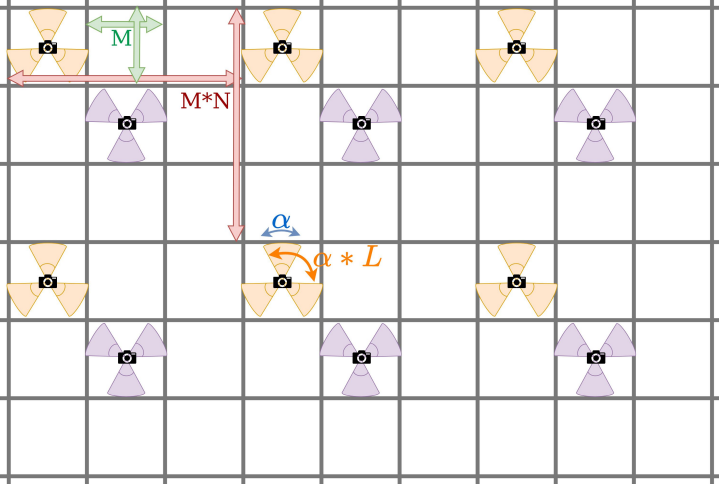
\includegraphics[width=0.7\textwidth]{pics/Chapter2/cosplaceclassify.png}
    \caption{Minh họa cách phân loại dữ liệu của mô hình CosPlace \cite{berton2022rethinking}}
\end{figure}

\subsubsection{Học truy xuất thông qua học xếp hạng}

Truy xuất hình ảnh, tương tự với bài toán "học xếp hạng", là quá trình học thông số và tìm phương thức truy xuất đặc trưng tốt nhất để biểu diễn sự tương quan giữa các phần tử trong tập dữ liệu dựa trên một hàm tính toán tương quan (distance function). Phần lớn các hướng tiếp cận cho bài toán nhận diện địa điểm trực quan sửa dụng một trong hai hàm mất mát chính với cùng ý tưởng:

\begin{itemize}
    \item hàm mất mát tương phản (contrastive loss), sử dụng các mạng nơ-ron siamese \cite{ong2017siamese, GeM, randenovic2016BoW}; và
    \item hàm mất mát ba phần tử (triplet loss), sử dụng các mạng nơ-ron có ba phần tử \cite{arandjelovic2016netvlad, gordo2016deep, gordo2017endtoend, wang2014learning, jin2017learned, zheng2018sift}.
\end{itemize}

Với mỗi mẫu dữ liệu huấn luyện, mô hình học truy xuất thông qua học xếp hạng được cung cấp những mẫu dữ liệu tích cực hoặc tiêu cực. Hàm mất mát có nhiệm vụ huấn luyện các đặc trưng sao cho những mẫu dữ liệu có giá trị tích cực sẽ có đặc trưng mang khoảng cách nhỏ và những mẫu dữ liệu có giá trị tiêu cực có khoảng cách lớn. Dưới góc nhìn của bài toán nhận diện địa điểm trực quan, một mẫu dữ liệu tích cực là ảnh ở cùng vị trí địa lý với ảnh huấn luyện, trong khi một mẫu dữ liệu tiêu cực là ảnh ở một vị trí địa lý khác. Các mô hình học truy xuất thông qua học xếp hạng có thể được chia thành hai nhóm chính: học truy xuất thông qua hàm mất mát tương phản và học truy xuất thông qua hàm mất mát ba phần tử. Như đã nhắc đến, để thực hiện quá trình học truy xuất thông qua học xếp hạng, các mô hình học truy xuất cần thực hiện quá trình khai phá thông tin tương quan (example mining) trong quá trình huấn luyện. Hướng tiếp cận này cho phép các nhà nghiên cứu phát triển các mô hình học giám sát yếu \cite{arandjelovic2016netvlad, jin2017learned} và học không giám sát \cite{radenovic2018fine} bằng cách lợi dụng các thông tin định vị để hỗ trợ quá trình khai phá. Tuy nhiên, quá trình khai phá này có chi phí tính toán cao, giới hạn thời gian và phạm vi dữ liệu có thể sử dụng để huấn luyện mô hình. \cite{arandjelovic2016netvlad} đánh dấu bước phát triển quan trọng trong hướng tiếp cận và đề xuất các hướng phát triển để tối ưu hóa quá trình này:

\begin{itemize}
    \item Lấy mẫu (Sampling): Hàm mất mát chỉ được tính cho tập hợp các mẫu dữ liệu tiêu cực và mỗi bước lấy mẫu sẽ thừa hưởng kết quả của những mẫu dữ liệu mang giá trị tiêu cực lớn nhất.
    \item Lưu đệm (Caching): Những đặc trưng được lưu trữ trong bộ nhớ đệm và chỉ được tính toán lại sau một số bước lấy mẫu huấn luyện nhất định tùy thuộc và tần suất học của mô hình (learning rate).
    \item Phân cụm (Clustering): Những đặc trưng được phân cụm dựa theo giá trị vị trí GPS thành các cụm nhỏ hơn và các mẫu huấn luyện trong cùng cụm sẽ chia sẻ cùng mẫu dữ liệu tiêu cực.
\end{itemize}


\subsection{Tìm kiếm tương đồng}
Bước thứ hai trong quy trình truy xuất ảnh thường là tác vụ tìm kiếm k lân cận gần nhất, hay nói là cách khác là tìm ra k ảnh có sự tương đồng cao nhất với ảnh nhận vào từ cơ sở dữ liệu. Tuy đơn giản về bản chất nhưng đây lại là tác vụ cực kỳ tốn kém về mặt tài nguyên đặc biệt là trong những bài toán với số chiều lớn. Một số nghiên cứu đã tăng tốc quá trình tìm kiếm bằng việc sử dụng các phương pháp tìm kiếm lân cận xấp xỉ (ANN) - không tiến hành quét cạn, sử dụng các kiến trúc chỉ mục khác,... \cite{4270175, Xie2015ImageCA, Mikolajczyk2007ImprovingDF, Muja2009FastAN, Muja2012FastMO, wang2017survey, magliani2019efficient, johnson2017billionscale}.

Với bước truy xuất ảnh, một yếu tố quan trọng cần cân nhắc chính là điều kiện bộ nhớ cần thiết của các phương pháp tìm kiếm - các biểu diễn ảnh quá lớn sẽ dẫn đến tiêu tốn cực nhiều tài nguyên của cơ sở dữ liệu. Để giải quyết vấn đề này, các nhà nghiên cứu có xu hướng hướng đến việc cải thiện tác vụ tìm kiếm tương đồng về mặt ổn định cũng như khả năng mở rộng. Các cấu trúc chỉ mục dựa trên tệp đảo ngược \cite{Salton1988TermWeightingAI} đã được sử dụng để thực hiện tìm kiếm không quét cạn, đặc biệt hiệu quả với các biểu diễn véc-tơ thưa \cite{Johns2011FromIT, Sivic2003VideoGA, imageSearchKernel, Mohedano2016sOL, noh2018largescale, Philbin2007ObjectRW}. Trong \cite{Johns2011FromIT}, thời gian truy xuất được giảm bằng cách nhóm các hình ảnh cơ sở dữ liệu tương tự và sau đó thực hiện việc ghép tương đồng theo cụm. Các kỹ thuật lượng tử hóa như k-means \cite{Philbin2007ObjectRW, Torii2013VisualPR}, nhị phân hóa \cite{Perronnin2010LargescaleIR} và lượng tử hóa tích \cite{imageSearchKernel} cũng được áp dụng để giảm yêu cầu bộ nhớ lưu trữ dữ liệu, các kỹ thuật này còn được kết hợp với tính toán khoảng cách không đối xứng \cite{5432202} và phép gán bội \cite{imageSearchKernel, Jgou2008HammingEA, 5432202, Philbin2007ObjectRW, Tolias2014VisualQE, Li2015PairwiseGM} để giảm thiểu tối đa lỗi lượng tử hóa. Kỹ thuật chỉ mục đảo cũng đã được tổng quát hóa để làm việc với lượng tử hóa tích \cite{Guo2016DeepLF, 5432202, Babenko2012TheIM}, cải thiện thêm tốc độ và độ chính xác của phép tìm kiếm, với một chi phí bộ nhớ tương đối nhỏ.

\subsection{Các mô hình truy xuất địa danh khác}
Các phương pháp nhận diện địa điểm trực quan thường được nghiên cứu theo xu hướng sử dụng ngữ cảnh của các ảnh trên đường phố. Việc có quyền truy xuất vào ảnh vệ tinh cũng như sự khuếch tán của rô-bốt trên không được trang bị camera đã mở ra một hướng phát triển mới. Một mặt, ảnh vệ tinh cho phép chúng ta có được đa dạng các góc nhìn cũng như một góc nhìn rộng hơn của khu vực. Mặt khác, chúng mở ra những thách thức như thiếu sót chi tiết trực quan.

\subsubsection{Định danh từ xa}
Trong truy xuất ảnh định danh từ xa, cũng như trong các tác vụ VPR cổ điển, mục đích vẫn là xác định vị trí ảnh nhận vào thông qua việc truy xuất ảnh tương đồng từ cơ sở dữ liệu. Do ảnh được chụp từ máy ảnh hướng xuống được trang bị trên một thiết bị bay hoặc từ vệ tinh dẫn đến việc ảnh sẽ phản ánh một khu vực địa lý lớn với nhiều vật thể có kích thước khác nhau. Các yếu tố vật thể dễ phân biệt ở tầng mặt đất như các tòa nhà lại không mang nhiều thông tin khi nhìn từ phía trên cao. Mặt khác, các yếu tố không mang quá nhiều thông tin hữu ích ở tầng mặt đất như đường xá lại quan trọng trong tác vụ định danh từ xa.

Dù cho có nhiều sự bất tương đồng, đã có những phương pháp VPR cổ điển được áp dụng để giải quyết bài toán định danh từ xa. Trong \cite{Tang2018UnsupervisedDF}, tác giả đề xuất sử dụng một phương pháp dựa trên túi-từ. Đầu tiên, các hình ảnh được chia thành các phân vùng sử dụng các phương pháp khác nhau. Sau đó, biểu diễn hình ảnh được xây dựng bằng cách kết hợp các đặc trưng ngầm được trích xuất bằng cách đưa mỗi phân vùng qua phần mã hóa của một mạng tích chập học sâu. Cuối cùng, túi-từ được tạo ra bằng cách sử dụng những biểu diễn này. Thay vì sử dụng phân vùng - tốn kém về mặt tài nguyên tính toán, \cite{Imbriaco_2019} đề xuất sử dụng kiến trúc DELF để trích xuất các đặc trưng cục bộ đáng chú ý sau đó kết hợp chúng thông qua trình tổng hợp VLAD. Ngoài ra, vì xác minh hình học khó áp dụng cho hình ảnh định dạng từ xa, các nhà nghiên cứu sử dụng mở rộng truy vấn dựa trên vector bộ nhớ \cite{7870636} để cải thiện kết quả truy vấn.

\begin{figure}[H]
    \centering
    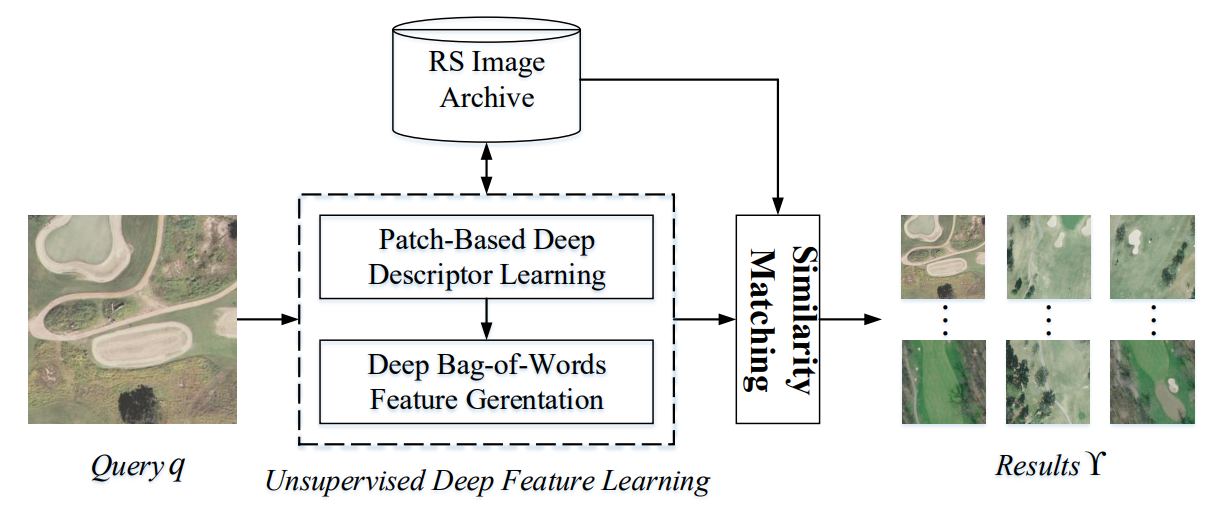
\includegraphics[width=\textwidth]{pics/Chapter2/rsir.png}
    \caption{Minh họa mô hình DBOW \cite{Tang2018UnsupervisedDF}}
\end{figure}

\subsubsection{Truy xuất vị trí từ các góc nhìn chéo (cross-view geo-localization)}
Một công dụng khác của ảnh trên không được sử dụng trong nhận diện địa điểm trực quan là truy xuất vị trí từ các góc nhìn chéo. Cụ thể với hướng tiếp cận này, ảnh nhận vào sẽ ở mức độ mặt đất và ảnh từ cơ sở dữ liệu sẽ là ảnh trên không. \cite{Lin2015LearningDR} xem xét trường hợp cụ thể trong đó các hình ảnh trên không được lấy từ cơ sở dữ liệu Google Street View và được chụp với góc khoảng 45 độ cùng với bản đồ độ sâu thô. Thông tin này, cùng với giả định của mô hình máy ảnh trực giao, cho phép chiếu lại các hình ảnh tầng mặt đất lên tầng trên không và thiết lập các kết nối mặt đất-trên không. Những kết nối này sau đó được sử dụng như các mẩu dữ liệu để đào tạo một bộ trích xuất đặc trưng dựa trên CNN với mất mát đối lập. \cite{workman2015widearea} đề xuất huấn luyện một mô hình nơ-ron tích chập để trích xuất biểu diễn kết nối đầy đủ của các hình ảnh trên không bằng cách sử dụng một hàm mất mát $l_2$ để căn chỉnh những biểu diễn này với những biểu diễn được trích xuất từ mô hình đã được huấn luyện trước cho các hình ảnh mặt đất tương ứng. Góc nhìn chéo cũng được tận dụng trong \cite{Castaldo2015SemanticCM} cho trường hợp của hình ảnh hệ thống thông tin địa lý gắn với bản đồ ngữ nghĩa. Tương tự như \cite{Lin2015LearningDR}, một phép chiếu lại được sử dụng để chỉnh sửa hình ảnh tầng mặt đất, nhưng phép chiếu lại được áp dụng cho một bản sao có được phân chia ngữ nghĩa của ảnh truy vấn.

\begin{figure}[H]
    \centering
    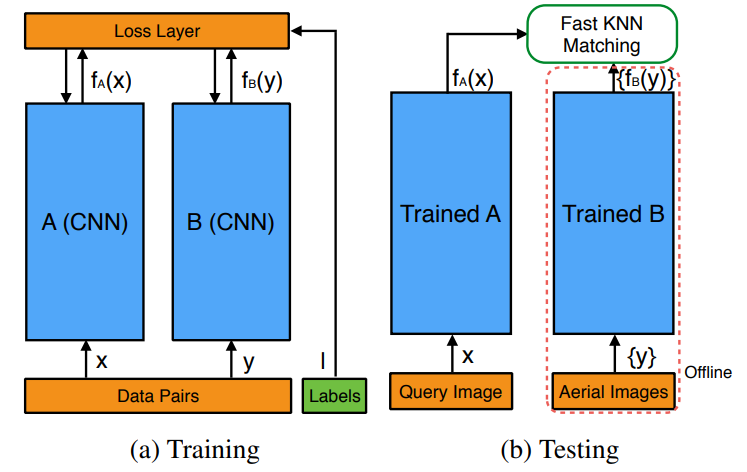
\includegraphics[width=\textwidth]{pics/Chapter2/wherecnn.png}
    \caption{Minh họa mô hình DBOW \cite{Lin2015LearningDR}}
\end{figure}

\subsection{Các khó khăn so với bài toán truy xuất hình ảnh cơ bản}

Mặc dù bài toán truy xuất địa danh thường được đánh giá và phát triển dưới góc nhìn là một bài toán truy xuất hình ảnh hoặc truy xuất instance, để biến đổi các giải pháp cho bài toán truy xuất hình ảnh thành giải pháp cho bài toán này, chúng ta cần phải đề xuất các hướng phát triển để triệt tiêu các khó khăn gắn liền với bản chất của dữ liệu địa danh. Khi nhận diện dữ liệu địa danh trong tập dữ liệu huấn luyện thành thị, mô hình học sâu sẽ phải xử lý một lượng lớn dữ liệu chứa các yếu tố lặp đi lặp lại đến từ kiến trúc nhân tạo như đường phố và cơ sở hạ tầng. Khi xử lý dữ liệu được thu thập trong một khoảng thời gian dài, mô hình học sâu cần đảm bảo tính bền của các đặc trưng biểu diễn trước các yếu tố thay đổi về điều kiện môi trường và phông cảnh được tạo ra do nhiều yếu tố phức tạp như mùa màng, thời tiết, thời gian, ánh sáng, \dots. Ngoài ra, dữ liệu đại diện cho các đối tượng địa danh mà mô hình cần học thường được thu thập từ các góc nhìn khác nhau với thiết bị và cảm biến khác nhau, yêu cầu khả năng khái quát hóa cao của mô hình học sâu. Quá trình phát triển để tăng cường độ bền của đặc trưng biểu diễn trước thay đổi trong điều kiện tự nhiên, môi trường, xã hội, thiết bị thu thập dữ liệu đã đặt bài toán truy xuất địa danh vào một phân loại khác biệt so với bài toán truy xuất hình ảnh cơ bản. Trong phần này, chúng tôi sẽ trình bày các khó khăn đặc trưng của bài toán truy xuất địa danh và các hướng phát triển để giải quyết các khó khăn này, lấy cảm hứng từ các giải pháp đã được đề xuất cho bài toán truy xuất hình ảnh cơ bản và các bài toán khác.

\subsubsection{Chọn vật thể và góc nhìn}

Tập dữ liệu hình ảnh địa danh cần xử lý trong bài toán truy xuất địa danh mang nhiều yếu tố lộn xộn (clutter), gây nhiễu, tạo ra hiện tượng phân tâm (visual distractors) cho các mô hình. Từ những ngày đầu phát triển, các nhà nghiên cứu đã ghi nhận mức độ quan trọng của quá trình quan sát và chọn ra các thành phần, góc nhìn của ảnh mang giá trị thông tin cao và tránh các yếu tố gây nhiễu, giảm hiệu năng\cite{4270175, knopp2010avoiding, predicting-good-features, Torii2013VisualPR, arandjelovic2015dislocation}. Đến nay, các hướng tiếp cận thường tối ưu hóa quá trình này theo hai chiến lược chính:

\begin{enumerate}
    \item Chọn vùng (region selection)
    \item Cơ chế tập trung (attention) và lớp trọng số (weighting)
\end{enumerate}

Chọn vùng là một chiến lược để xử lý vấn đề cluterring và visual distractors. Bằng cách chọn ra các vùng trong ảnh mang giá trị thông tin cao, mô hình truy xuất so sánh tương quan giữa các đặc trưng biểu diễn trích xuất được từ các vùng khác nhau thay vì giữa các ảnh khác nhau, trên lý thuyết, dẫn đến hiệu năng cao và tính bền bỉ cho mô hình. Trên thực tế, tuy đạt được độ bền cao so với thay đổi về tỉ lệ và thay đổi góc nhìn, việc trích xuất các vùng ảnh trực tiếp từ ảnh đầu vào được đánh giá là kém hiệu quả và tốn nhiều tài nguyên tính toán. Một hướng tiếp cận khác sử dụng mạng học sâu tích chập, chia ảnh đầu vào bằng một lưới với kích thước cố định và trích xuất vùng ảnh từ các đặc trưng trích xuất được\cite{razavian2016visual, tolias2015particular}. Phướng tiếp cận này làm giảm được số lượng tham số cần học, tuy nhiên không giải quyết được vấn đề đã nhắc đến một cách hiệu quả. Kích thước lưới được quyết định một cách cố định và mà không tận dụng được bối cảnh của ảnh, dẫn đến số lượng các vùng ảnh được chọn không mang ý nghĩa tương đương với các vùng ảnh mang ý nghĩa bất kể độ mịn của lưới. Đồng thời, việc tăng độ mịn của lưới với mục tiêu tăng cường độ bền của mô hình sẽ làm tăng đáng kể số lượng các vùng ảnh được trích xuất, dẫn đến tăng đáng kể thời gian tính toán và số lượng tham số cần học, cho thấy rằng đây không phải là một hướng tiếp cận thân thiện với phạm vi lớn. Đề xuất các hướng giải quyết cho vấn đề này, các mô hình R-MAC\cite{tolias2015particular} được chỉnh sửa với các mạng đề xuất vùng tương tự với hướng tiếp cận được đề xuất trong Faster R-CNN\cite{ren2015faster} và mô hình ASMK aggregation\cite{selective-match-kernel} với cơ chế truy xuất sử dụng MobileNet V2\cite{sandler2018mobilenetv2, teichmann2019detect}. Ngoài ra, nhận thấy các lớp gần cuối của mạng học sâu tích chập thường thể hiện các đặc trưng ngữ nghĩa có ý nghĩa\cite{ZeilerVisualizingAU}, các hướng tiếp cận hiện đại thường khai thác trực tiếp đặc trưng từ các lớp sau của mạng tích chập cho tác vụ chọn vùng\cite{chen2017only, khaliq2019holistic}.

Cơ chế attention và lớp trọng số là một chiến lược mới, với mục tiêu chọn ra những thông tin, đặc trưng mang tính tương quan cao từ các hình ảnh để tăng hiệu năng hoạt động của các mô hình truy xuất địa danh. Khác với cơ chế chọn vùng, cơ chế attention không truy xuất thông tin từ những vùng mà mô hình cho là quan trọng, mà truy xuất tất cả các vùng trong ảnh cùng một lúc. Sau đó, các đặc trưng trích xuất được được tổng hợp lại dựa theo một lớp trọng số và điều kiện đánh giá cụ thể. Điều kiện đánh giá này, vào những ngày đầu, được thiết kế dựa theo các cơ chế phỏng đoán (heuristic) như khoảng cách so với trọng tâm hình ảnh, độ nổi bật của đặc trưng trong tất cả các kênh (channel), \dots. Hướng tiếp cận này đạt nhiều thành công trong các tập dữ liệu chứa các đối tượng lặp đi lặp lại và thiếu tính tương phản cao. Ngoài ra, sự đa dạng trong phương thức thiết kế lớp trọng số cho phép nhà nghiên cứu tùy chỉnh mô hình để giải quyết các vấn đề cụ thể. Tuy nhiên, các mô hình này dễ trở nên thiếu linh hoạt, khó huấn luyện để tổng quát hóa và chỉ đạt kết quả tốt nhất khi được huấn luyện đầu-cuối (end-to-end). Ngày nay, hướng tiếp cận này thường được hiện thực sử dụng cơ chế Transformers (một loại mô hình auto-encoder), Vision Transformers (ViT)\cite{dosovitskiy2020image}, \cite{shavit2023coarse}. Nhận thấy tác động tài nguyên của ViT, \cite{alibey2023mixvpr} đề xuất sử dụng mạng học sâu MLP-Mixer\cite{tolstikhin2021mlpmixer}, một mạng học sâu sử dụng nhiều lớp MLP (Multi-Layer Perceptron) kết nối đầy đủ (fully-connected) với nhau, để thay thế cho ViT với mục tiêu đạt được cùng hiệu năng nhưng đòi hỏi ít tài nguyên hơn. Tác giá của \cite{alibey2023mixvpr} cho rằng, cho tác vụ truy xuất địa danh, MLP-Mixer là một lựa chọn có tiềm năng cao để thay thế cho ViT.

\subsubsection{Góc nhìn ảo và sự biến dạng}

Trong thực tế, các đặc trưng cục bộ dày đặc được sử dụng cho quá trình so sánh tương quan, mặc dù mạnh mẽ hơn so với các đặc trưng cục bộ thưa thớt trước các thay đổi về ánh sáng \cite{zhou2016evaluating}, không thu hẹp được các ảnh hướng đến từ biến đổi hình học (tỷ lệ và góc nhìn). Đối mặt với vấn đề này, một số bài báo \cite{torii201524, taira2018inloc} đề xuất các chiến thuật sinh góc nhìn (view synthesis). Dựa vào cơ sở dữ liệu chứa ảnh RGB và thông tin độ sâu, các mô hình này truy xuất một danh sách các ví trí sơ bộ gần đúng và chế tạo góc nhìn ảo tương ứng, đưa ảnh truy vẫn và ảnh truy xuất về cùng một góc nhìn. Quá trình lựa chọn ảnh khớp tốt nhất được thực hiện một cách đơn giản, trực tiếp lên số lượng các điểm ảnh trùng và không trùng của các ảnh. Mặc dù hướng tiếp cận này tạo ra số lượng lớn các dị vật trong ảnh (visual artifacts), chiến thuật này thường đạt kết quả tốt hơn so với các mô hình truy xuất địa danh cơ bản.

Ngoài ra, trong các ứng dụng đặc biệt hơn như truy xuất vị trí từ các góc nhìn chéo, các mô hình cần phải truy vấn ảnh lấy được từ các góc nhìn trên không để so sánh với ảnh lấy được từ góc nhìn trên mặt đất và ngược lại. Sự khác nhau rất lớn về góc nhìn này đã tạo nên không ít khó khăn. Một giải pháp cho vấn đề này là quá trình chiếu tất cả các ảnh về một góc nhìn chung \cite{lin2015learning, castaldo2015semantic}. Một giải pháp khác sử dụng thêm các đặc trưng chỉ hướng (rolling descriptor) cho quá trình truy vấn để mã hóa thông tin chỉ hướng vào đặc trưng biểu diễn của các ảnh trong cơ sở dữ liệu \cite{xia2023convolutional}. Trong quá trình suy luận (inference), mô hình này khai phá thông tin chỉ hướng từ các ảnh góc rộng (panorama) để mã hóa vào biểu diễn truy vấn, so sánh tương quan giữa các đặc trưng biểu diễn này với các đặc trưng biểu diễn của các ảnh trong cơ sở dữ liệu.

\subsubsection{Thông tin ngữ nghĩa}

Việc thu thập và sử dụng thông tin ngữ nghĩa được đánh giá rất cao trong các hướng tiếp cận của bài toán. Thông tin này hỗ trợ trực tiếp quá trình chọn vùng và các điểm ảnh quan trọng như một yếu tố heuristic, cho phép các mô hình phát triển độ bền vững của mình trước các tác động môi trường và thay đổi trong điều kiện khách quan. Các hướng tiếp cận hiện đại ngay nay thường sử dụng triệt để mọi thông tin mà môi trường truy xuất cung cấp như thông tin về độ sâu, thông tin về mùa màng, thời gian, ánh sáng, \dots Ngoài ra, các loại thông tin như độ liên quan giữa số lượng, sự hiện diện của các phương tiện giao thông, các kiến trúc lặp đi lặp lại cũng hỗ trợ đáng kể cho quá trình lọc đặc trưng, loại bỏ các yếu tố gây nhiễu, lựa chọn các cột mốc địa danh có tính tương quan cao.

\subsubsection{Thông tin về độ sâu}

Thông tin độ sâu thường được xem là dữ liệu đi kèm với các tập dữ liệu truy xuất địa danh. Đóng vai trò là cầu nối giữa hình ảnh hai chiều và thông tin ba chiều của địa danh, thông tin độ sâu thường được sử dụng để tăng độ bền cho các mô hình học sâu trước các thay đổi về điều kiện ảnh. Ngoài ra, độ sâu còn có thể được tích hợp vào các đặc trưng biểu diễn để hỗ trợ quá trình trích xuất biểu diễn toàn cục cho quá trình truy xuất hình ảnh. Tuy nhiên, giống với các mô hình học từ dữ liệu thu thập được từ cảm biến độ sâu như LiDAR, việc đòi hỏi dữ liệu huấn luyện chứa thông tin về độ sâu là một hạn chế lớn, giảm khả năng mở rộng cho tập dữ liệu vì các vấn đề thu thập, lưu trữ, cập nhật và huấn luyện. Vì lý do này, một số hướng tiếp cận trong bài toán thường thiết kế các mô đun học sâu phụ cho mô hình của mình, với mục đích tự xây dựng lại một phiên bản cơ bản hơn của thông tin này trong quá trình huấn luyện. Sử dụng phương pháp tiếp cận này, mô hình chỉ cần nhận vào ảnh 2 chiều RGB trong quá trình truy xuất\cite{piasco2019learning}.

\subsubsection{Thích nghi với điều kiện môi trường thay đổi}

Những thách thức mà các mô hình truy xuất địa danh phải đối mặt khi đối mặt với các thay đổi về điều kiện môi trường như ánh sáng, thời tiết và mùa màng được công nhận rộng rãi\cite{zaffar2019levelling} và vẫn còn đươc xem là một vấn đề mở. Một lượng lớn các tài liệu nghiên cứu đã nghiên cứu các hạn chế của các đặc trưng học sâu trong các điều kiện khó khăn \cite{zhou2016evaluating, sunderhauf2015performance, chen2017deep} và các phân tích này đã cung cấp một số hướng dẫn để tìm ra các đặc trưng mạnh mẽ hơn. Các nhà nghiên cứu cho rằng, các đặc trưng cục bộ cần phải được phân bố một cách dày đặc mới có thể tránh khỏi vấn đề hiệu năng kém trước các thay đổi về độ sáng (ngày/đêm). Đồng thời, một giải pháp thay thế hiệu quả là quá trình tiền xử lý dữ liệu ảnh đầu vào bằng một mô hình học sâu đơn giản, với mục tiêu chuẩn hóa độ sáng của ảnh. Một số đánh giá xếp hạng cho thấy, các đặc trưng học sâu có hiệu năng tốt hơn trước khi được so sánh với các đặc trưng được thiết kế thủ công\cite{arandjelovic2017netvlad}. \cite{taira2018inloc} ghi nhận rằng đặc trưng cục bộ dày đặc hoạt động tốt trong môi trường trong nhà, nơi thiếu các đặc trưng lặp đi lặp lại và đặc trưng bề mặt vật liệu (texture) trong khi các mô đun trích xuất đặc trưng (feature extractions) hoạt động tốt hơn trong môi trường ngoài trời, khai thác các yếu tố ít thay đổi như kiến trúc và đặc điểm của đường phố. Một số hướng phát triển có tiềm năng sử dụng các mô hình có cơ chế tập trung lên những phần nhỏ của một ảnh như \cite{sunderhauf2015place, chen2017only, khaliq2019holistic} sử dụng chiến thuật vùng hấp dẫn (regions of interest), \cite{zhu2018attention, chen2017only, khaliq2019holistic, wang2019atloc, wang2022transvpr, alibey2023mixvpr} sử dụng cơ chế attention, \cite{garg2018lost, naseer2017semantics, seymour2019semantically}. Đồng thơi, sử dụng một chuỗi các hình ảnh liên tực thay cho một hình ảnh đơn lẻ cũng có tác động lớn đối với độ bền của mô hình trước điều kiện mô hình thay đổi \cite{naseer2018robust, hausler2019multi, hong2019textplace, chancan2020hybrid}.

Các giải pháp cho vấn đề thay đổi điệu kiện môi trường thường phải sử dụng các chiến thuật có yêu cầu tài nguyên lớn, khó phát triển quy mô. \cite{doan2019scalable} đề xuất một giải pháp ba bước để khắc phục các vấn đề này: xây dựng mô hình chứa cơ sở dữ liệu có thể tiếp tục mở rộng phạm vi với nhiều ảnh được thu thập ở các điều kiện môi trường khác nhau. Doan và nnk đề xuất mô hình:

\begin{enumerate}
    \item Một thuật toán nhận diện địa điểm trực quan được xây dựng dựa trên mô hình Markov ẩn (Hidden Markov Model) với hiệu năng huấn luyện và kiểm thử cao.
    \item Một chiến thuật chọn lọc điều chỉnh số lượng ảnh được thêm vào cơ sở dữ liệu, đảm bảo chỉ thêm các ảnh biểu diễn các ảnh với dữ liệu mới và chứa nhiều đặc điểm quan trọng.
    \item Một thuật toán nén hợp nhất các phần kết nối được với nhau trong cơ sở dữ liệu, giảm kích thước lưu trữ.
\end{enumerate}

Gần đây hơn, một số nghiên cứu tìm cách đối mặt với vấn đề này dưới góc nhìn khác, giải quyết vấn đề miền chéo, khi ảnh truy vấn chứa nhiều sự khác biệt về độ sáng, thời tiết, mùa màng hoặc thiết bị thu thập ảnh so với ảnh trong cơ sở dữ liệu. Hướng tiếp cận này đặt ra mục tiêu sinh ra ảnh mới để thay thế ảnh truy vấn, cùng mô tả một cảnh nhưng với với miền của ảnh trong cơ sở dữ liệu. Trong \cite{Porav2018AdversarialTF, Annosheh2019Night} quá trình sinh ảnh thường được thực hiện bởi mạng đối nghịch tạo sinh (GAN). Thay vì căn chỉnh dữ liệu các miền khác nhau, một hướng tiếp cận khác đặt trọng tâm trong quá trình học đặc trưng đa miền và tách cụm những đặc trưng phụ thuộc vào điều kiện môi trường và những đặc trưng bất biến \cite{yin2019multi}. Mạng đối nghịch tạo sinh đạt hiệu quả đáng kể đối với các vấn đề miền chéo chứa sự khác biệt về độ sáng, thời tiết hoặc mùa màng nhưng chưa giải quyết được vấn đề miền chéo chứa sự khác biệt về thiết bị thu thập. Trong thực tế, các tập dữ liệu huấn luyện mô hình luôn được thu thập trong khoảng thời gian sớm hơn so với dữ liệu truy vấn. \cite{wang2019attention} đề xuất kiến trúc sử dụng một mô hình trích xuất đặc trưng học sâu tích chập với lớp aggregation VLAD \cite{jegou2010aggregating} và hai mô đun chủ chốt:

\begin{itemize}
    \item một mô đun attention đánh giá độ quan trọng của các đặc trưng tổng hợp được từ lớp VLAD, và
    \item một hàm mất mát thích nghi miền sử dụng hàm khác biệt trung bình tối đa đa hạt nhân (multi-kernel maximum mean discrepancy hoặc MK-MMD) hỗ trợ mạng học được không gian chung của mà cả hai miền.
\end{itemize}

Trong đó, mô đun attention được đánh giá có cống hiến ít so với cải tiến chung của mô hình trong khi hàm mất mát nắm vị trí trọng tâm.

Thêm vào đó, đặt vấn đề dưới góc nhìn là quá trình thu thập dữ liệu, \cite{hu2020dasgil} đề xuất sử dụng tập dữ liệu ảo chứa thông tin độ sâu và thông tin ngữ nghĩa để huấn luyện mô hình học sâu. Quá trình huấn luyện lấy cảm hứng từ mô hình đối nghịch đảm bảo đặc trưng trích xuất được từ miền ảo và miền ảnh thật có độ phân bố tương tự nhau.

Trong [Adaptiveattentive geolocalization from few queries: A hybrid approach], Berton và nnk chứng minh hướng tiếp cận áp dụng kết hợp cả bài toán sinh dữ liệu (generative) và bài toán thích ứng miền (domain adaptation) có khả năng tăng hiệu năng của các mô hình cao.



\section{Ước tính vị trí của máy ảnh - Pose Estimation}

Ước tính vị trí máy ảnh (Camera Pose Estimation) là một bài toán thuộc chuyên ngành thị giác máy tính nhằm xác định vị trí (position) và góc quay (orientation) chính xác nhất có thể của máy ảnh thông qua dữ liệu hình ảnh được chụp từ chính máy ảnh. Đây là một bước cực kỳ quan trọng trong việc giải quyết bài toán định vị trực quan, thường được áp dụng sau khi bước nhận dạng địa điểm trực quan đã trích xuất được ảnh từ kho dữ liệu. Hiện nay, có tương đối nhiều hướng tiếp cận đối với bài toán này. Một trong những phương pháp phổ biến nhất là huấn luyện một mô hình học sâu để xác định 6 chiều tự do (Degree of Freedom) từ số ít ảnh (Absoblute Pose Regression và Relative Pose Regression) hoặc xây dựng một mô hình 3D từ tập dữ liệu có sẵn rồi tiến hành chuyển ảnh đầu vào sang các điểm 3D để dễ dàng so sánh và xác định vị trí (Structure From Motion).

\subsection{Hồi quy vị trí tuyệt đối - Absolute Pose Regression}

Hồi quy vị trí tuyệt đối (Absolute Pose Regression) hướng đến việc dự đoán vị trí và góc quay chính xác nhất của ảnh bằng một mô hình mạng nơ-ron tích chập thông qua việc cải thiện trọng số của mô hình. Tùy thuộc vào đầu vào của mô hình mà hồi quy vị trí tuyệt đối được chia thành ba hướng chính: hồi quy vị trí tuyệt đối với một ảnh, chuỗi ảnh hoặc đoạn phim.

\subsubsection*{Hồi quy vị trí tuyệt đối đơn ảnh - Absolute pose regression through single monocular image}
Với phương pháp hồi quy vị trí tuyệt đối thông qua một ảnh (Absolute pose regression through single monocular image), quy trình chung thường bao gồm: đầu vào - mạng - đầu ra. Đầu vào sẽ là một ảnh RGB với đầu ra là vị trí 6 độ tự do của máy ảnh. Thông thường, kiến trúc của mạng lưới tính toán sẽ bao gồm các thành phần như sau: bộ mã hóa, bộ định vị, bộ hồi quy.

\begin{figure}[H]
    \centering
    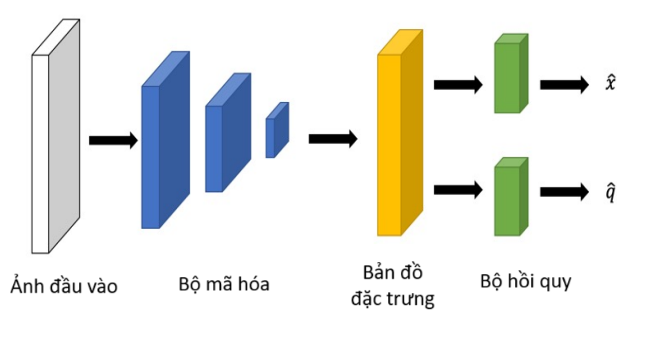
\includegraphics[width=\textwidth]{pics/Chapter2/kientruc_APR_1.png}
    \caption{Kiến trúc mô hình hồi quy vị trí tuyệt đối đơn ảnh \cite{kendall2016posenet}}
\end{figure}

\noindent\textbf{Phương pháp sử dụng hàm mất mát Euclidean cố định:}

PoseNet \cite{kendall2016posenet} là công trình đầu tiên huấn luyện mô hình mạng nơ-ron tích chập để hồi quy vị trí máy ảnh từ một ảnh RGB, hoàn toàn không phụ thuộc vào bất kỳ cơ chế bên ngoài nào khác. Vào thời điểm ra mắt, PoseNet đã cho thấy sự vững chắc của mô hình vượt trội so với phương pháp tái tạo kiến trúc từ chuyển động dựa trên cơ chế "biến đổi tính năng bất biến tỷ lệ" (Scale-invariant Feature Transform Structure from Motion): độ hiệu quả của kiến trúc vế sau giảm mạnh nếu độ lớn của tập dữ liệu huấn luyện giảm đến một mức nhất định. Hàm mất mát Euclidean của PoseNet được định nghĩa như sau:
\begin{center}
    $loss(I) = \left \| \hat{x} - x \right \|_2 + \beta \left \| \hat{q} - \frac{q}{\left \| q \right \|} \right \|_2$
\end{center}

Kế thừa từ PoseNet, đã có nhiều công trình và bài báo tìm cách cải thiện phương pháp định vị hoặc thay thế hàm mất mát nhằm nâng cao hiệu suất chung của toàn kiến trúc. Với các công trình có mong muốn cải thiện hàm mất mát của mô hình, một chiến thuật chung là kết hợp hàm mất mát Euclidean và phương pháp giảm độ dốc Stochastic. Về mặt cải thiện hiệu quả định vị cũng như tìm hiểu về độ thiếu chính xác của mô hình, một nhóm tác giả đề xuất thêm xác suất Bernoulli vào mô hình nơ-ron tích chập \cite{kendall2016modelling} nhằm xác định độ thiếu chính xác của mô hình. Ý tưởng chính của phương pháp này là xác định và tận dụng độ thiếu chính xác để dự đoán sai số trong định vị, phương pháp này đã cải thiện độ chính xác cho PoseNet cho cả những cảnh ngoài trời và bên trong nhà.
\begin{figure}[H]
    \centering
    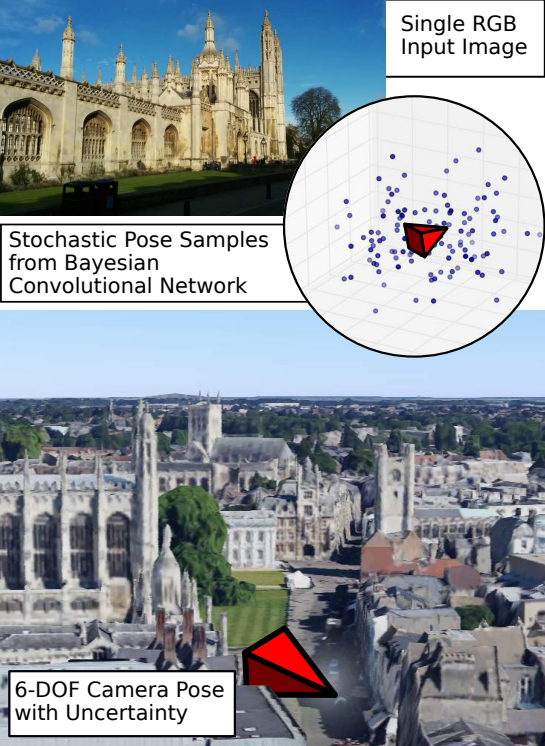
\includegraphics[scale=0.7]{pics/Chapter2/Ber_PoseNet.png}
    \caption{Minh họa mô hình CNN được áp dụng phân phối Bernoulli \cite{kendall2016modelling}}
\end{figure}
Từ những thông tin được nêu ra trong bài báo \cite{kendall2016posenet}, ta biết được rằng mô hình PoseNet có một lớp kết nối đầy đủ với 2048 chiều, tạo điều kiện cho việc áp dụng một lớp bộ nhớ dài ngắn hạn để giảm chiều đặc trưng giúp cải thiện độ chính xác định vị \cite{walch2017imagebased, wang2019atloc}. Nhóm tác giả Watch và cộng sự \cite{walch2017imagebased} đề xuất tận dụng các lớp bộ nhớ dài ngắn hạn lên đầu ra của PoseNet để giảm chiều và chọn ra những đặc trưng hữu ích nhất cho bài toán định vị vị trí. Các thí nghiệm đo lường cho thấy phương pháp này vượt trội hơn PoseNet khoảng 30\% về sai số vị trí và 55\% về sai lệch góc quay.
\begin{figure}[H]
    \centering
    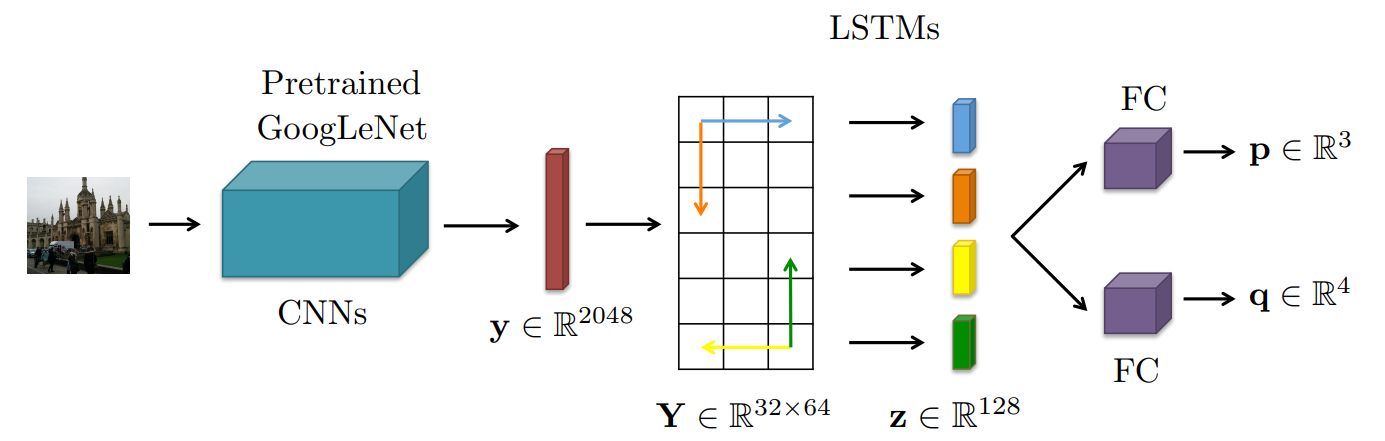
\includegraphics[width=\textwidth]{pics/Chapter2/LSTM_PoseNet.png}
    \caption{Minh họa kiến trúc mô hình LSTM PoseNet \cite{walch2017imagebased}}
\end{figure}
Để cải thiện độ chính xác định vị, một kiến trúc đồng hồ cát được đề xuất với việc thêm một phần chức năng mã hóa thông tin hữu ích từ kiến trúc vật thể thô và một phần chức năng thu chi tiết vật thể mịn. Hourglass PoseNet \cite{melekhov2017imagebased} có kiến trúc gồm ba thành phần chính là bộ mã hóa, bộ giải mã và bộ hồi quy. Mô hình này sử dụng một mô hình ResNet34 đã được tinh chỉnh làm bộ mã hóa - giải mã. SVS PoseNet \cite{deep-regression} dùng mô hình VGG16 kết hợp thêm hai lớp kết nối đầy đủ để có thể dự đoán riêng vị trí và góc quay. BranchNet \cite{7989663} sử dụng mô hình mạng hai nhánh học đồng thời biểu diễn góc quay và độ dời để giảm thiểu độ thưa của các vị trí được lấy mẫu một cách hiệu quả. Dù hướng tiếp cận có sự khác biệt, các công trình trên đều có cùng hàm mất mát với PoseNet.
\begin{figure}[H]
    \centering
    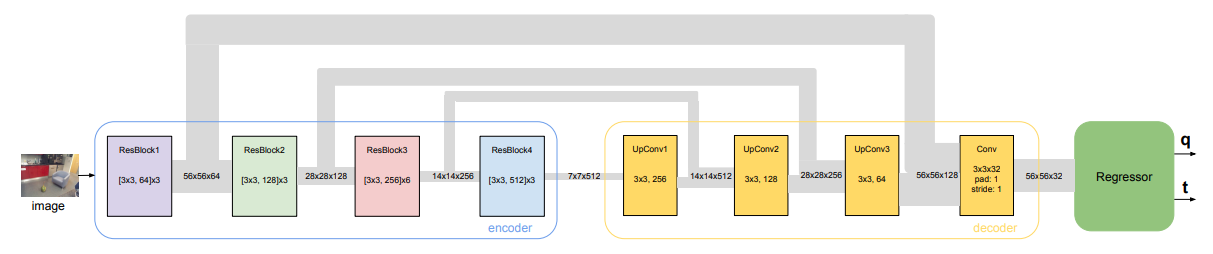
\includegraphics[width=\textwidth]{pics/Chapter2/hourglass_PoseNet.png}
    \caption{Minh họa kiến trúc mô hình Hourglass PoseNet \cite{melekhov2017imagebased}}
\end{figure}

\noindent\textbf{Phương pháp sử dụng hàm mất mát có trọng số học được:}

Để học được thông tin về vị trí và góc quay từ dữ liệu ảnh, hàm mất mát cố định Euclidean áp dụng các siêu tham số cân bằng để giúp việc học thông tin vị trí và góc quay một cách độc lập, tuy nhiên để học trọng số thì rất tốn kém. Geometric PoseNet \cite{kendall2017geometric} đề xuất sử dụng hàm mất mát vị trí có trọng số học được để cân bằng hiệu suất và cải thiện độ ổn định. Khi so sánh với PoseNet, phương pháp này giữ lại độ mở rộng và độ chắc chắn mà không cần chỉnh sửa các siêu tham số cố định cân bằng trong hàm mất mát.

AtLoc \cite{wang2019atloc} thêm vào mô hình một mô-đun tập trung (Attention Module) trước khi xác định các tọa độ hồi quy để ép buộc mạng phải tập trung vào phần chính - phần mang nhiều thông tin hữu ích nhất của hình ảnh đầu vào. Ngoài ra, AtLoc sử dụng ResNet34 được huấn luyện sẵn trên tập dữ liệu ImageNet làm bộ mã hóa, sau đó hồi quy lớp kết nối đầy đủ 2048 chiều của PoseNet.
\begin{figure}[H]
    \centering
    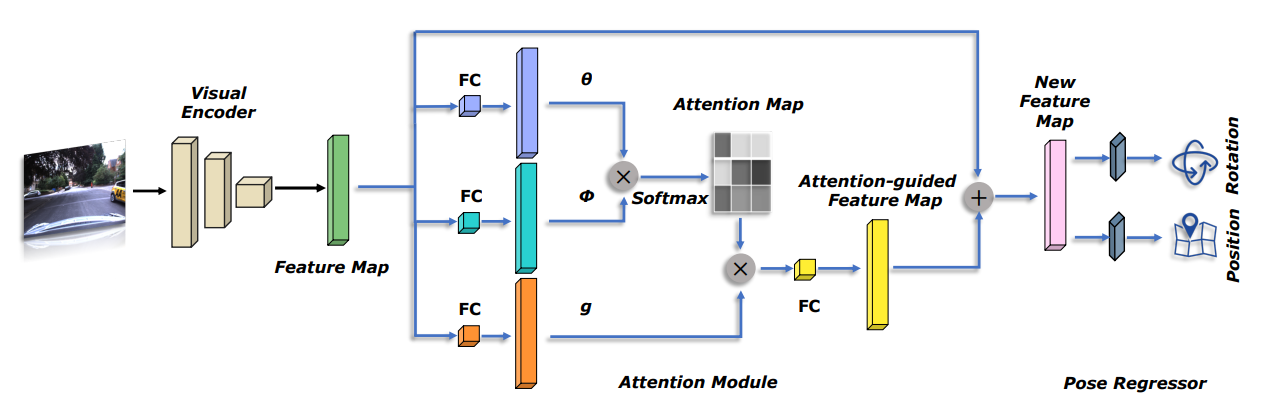
\includegraphics[width=\textwidth]{pics/Chapter2/atloc.png}
    \caption{Minh họa kiến trúc mô hình AtLoc \cite{wang2019atloc}}
\end{figure}
AdPR \cite{bui2019adversarial} thêm một mạng phân biệt và học đối lập. Điều này không chỉ hồi quy vị trí mà còn tinh chỉnh vị trí. Khi trích xuất đặc trưng, AdPR áp dụng mạng ResNet-18, vì nó có thể đạt được hiệu suất tốt nhất so với VGG16 và AlexNet. APANet \cite{chidlovskii2020adversarial} cũng sử dụng một mạng đối lập để tạo ra hình ảnh liên quan đến hình ảnh đầu vào để ước lượng tốt hơn vị trí của máy ảnh. Một mô-đun Dropout được thêm trước bộ mã hóa trích xuất đặc trưng để xuất ra nhiều khả năng không chắc chắn, điều này có thể cải thiện độ chắc chắn của mô hình dưới điều kiện thử thách như thay đổi vị trí, thời tiết,... . Sau khi trích xuất, mô-đun tập trung tự động được thêm để điều chỉnh lại trọng số bản đồ đặc trưng.
\begin{figure}[H]
    \centering
    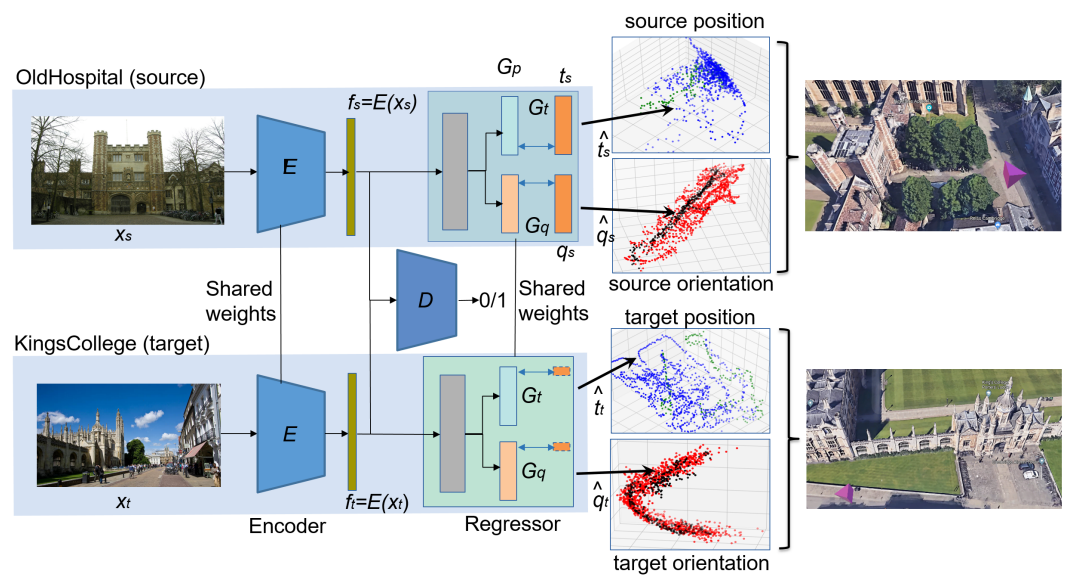
\includegraphics[width=\textwidth]{pics/Chapter2/apanet.png}
    \caption{Minh họa kiến trúc mô hình APANet \cite{chidlovskii2020adversarial}}
\end{figure}
\noindent\textbf{Phương pháp sử dụng hàm mất mát khác:}

Không dùng đến cả hàm mất mát cố định hoặc những hàm mất mát có trọng số học được, một số nhóm nghiên cứu đề xuất nên cân nhắc sử dụng các mô-đun khác để cải thiện hiệu suất định vị. GeoPoseNet \cite{kendall2017geometric} đề xuất sử dụng hàm mất mát tái chiếu: đặc tả sai sót tái chiếu của cảnh. Hàm mất mát tái chiếu chuyển mất mát chung học được thành khác biệt tọa độ ảnh, do đó có thể thay đổi trọng số giữa vị trí và góc quay, tùy thuộc vào các cảnh khác nhau trong quá trình huấn luyện mô hình. GPoseNet \cite{Cai2018AHP} xây dựng mô hình mới bằng cách thêm vào hai bộ "Hồi quy quá trình Gaussian suy luận biến phân ngẫu nhiên" (Stochastic Variational Inference Gaussian Process Regressions - SVI GPs) sau lớp kết nối đầy đủ để học phân phối xác suất của vị trí - hướng quay đầu ra và giảm tần suất sử dụng siêu tham số. Hàm mất mát của GPoseNet kết hợp hàm mất mát SVI GPs sử dụng ranh giới điều kiện dưới của hai xác suất tích lũy log $L_{s}vi$ và hàm mất mát CNN với siêu tham số $\beta_{g_{t}}$ và $\beta_{n_{q}}$ của PoseNet.
\begin{figure}[H]
    \centering
    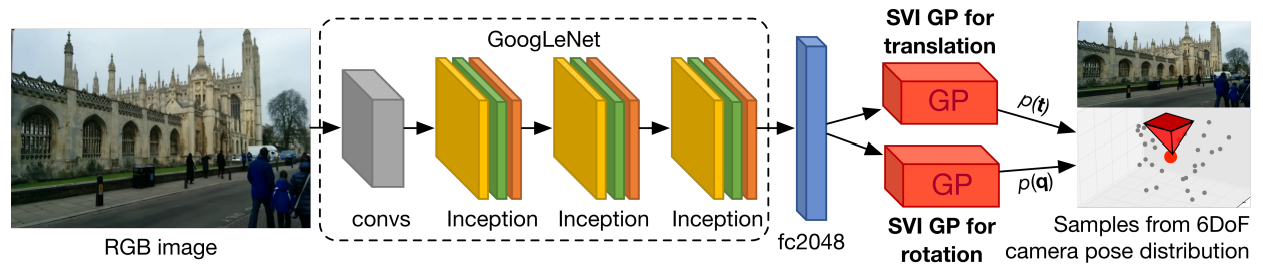
\includegraphics[width=\textwidth]{pics/Chapter2/gposenet.png}
    \caption{Minh họa kiến trúc mô hình GPoseNet \cite{kendall2017geometric}}
\end{figure}

Một nhóm nghiên cứu \cite{shavit2021learning, shavit2023coarse} đề xuất áp dụng mô hình Transformer vào tác vụ hồi quy vị trí tuyệt đối. Mô hình nhận vào một ảnh đơn và sử dụng một CNN làm bộ trích xuất đặc trưng, sau đó các bản đồ đặc trưng được truyền song song qua hai nhánh: mỗi nhánh là một mô hình Transformer đảm nhiệm một tác vụ riêng lần lượt là hồi quy vị trí và hồi quy hướng quay. Mô hình sử dụng hàm mất mát tương tự với PoseNet.
\begin{figure}[H]
    \centering
    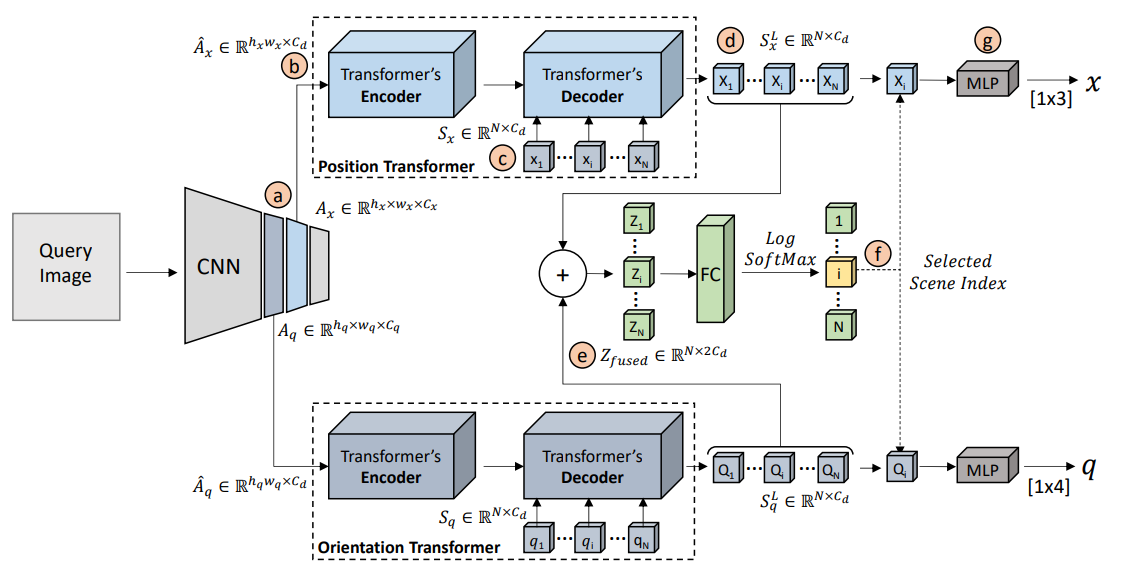
\includegraphics[width=\textwidth]{pics/Chapter2/trans.png}
    \caption{Minh họa kiến trúc mô hình Multi-Scene Transformer \cite{shavit2021learning, shavit2023coarse}}
\end{figure}

\subsubsection*{Hồi quy vị trí tuyệt đối đa ảnh - Absolute pose regression through auxiliary image sequence}
Một phương pháp khác được áp dụng để hồi quy vị trí tuyệt đối là áp dụng học có hỗ trợ với một chuỗi ảnh. Học có hỗ trợ được định nghĩa là phương pháp cải thiện hiệu suất của một tác vụ chính thông qua việc học cùng lúc các tác vụ hỗ trợ. Phương pháp học này giúp mô hình phát triển các biểu diễn dữ liệu tốt hơn. Bằng cách tận dụng các tác vụ hỗ trợ có liên quan khác trong quá trình học, hiệu suất của tác vụ chính có thể được cải thiện. Ở đây, học có hỗ trợ ám chỉ việc kết hợp APR với các tác vụ phụ có liên quan như đo lường cảm biến trực quan. Hàm mất mát của các phương pháp học có hỗ trợ thường bao gồm hàm mất mát của APR kết hợp với hàm mất mát của các phương pháp phụ trợ, thậm chí có thể kết hợp cả hàm mất mát của APR và RPR. Khác với các phương pháp hồi quy vị trí tuyệt đối đơn ảnh, phương pháp học có hỗ trợ học từ các cặp ảnh với bản chất là học cách xác định vị trí tuyệt đối bằng cách đánh giá trước hết vị trí tương đối với các ràng buộc phụ thuộc.

MapNet \cite{brahmbhatt2018geometryaware} đề xuất thêm một thuật ngữ mất mát lấy từ các cặp ảnh làm một ràng buộc hình học, điều này đã có thể cải thiện mạnh mẽ hiệu suất khả năng định vị. Về hàm mất mát, MapNet giảm thiểu tối đa cả mất mát vị trí tuyệt đối cho mỗi hình ảnh và mất mát vị trí tương đối giữa các cặp hình ảnh:
\begin{center}
    $l(I_{total}) = l(I_i) + \alpha\sum_{i\neq j}loss(I_{ij} )$
\end{center}
Trong đó, $loss(I_{ij} )$ ám chỉ vị trí máy ảnh tương đối $p_i$ và $p_j$ giữa các cặp hình ảnh $I_i$ và $I_j$, được tính bởi hàm mất mát với trọng số có thể học được.

Thêm vào đó, MapNet chuyển một giá trị quaternion thành logarit của giá trị đó - biểu diễn phép quay ba độ tự do (3DoF) với ba chiều chưa bị tham số hóa quá mức. $logq$ được biểu diễn như dưới đây, với $u$ và $v$ đại diện cho phần thực và ảo của một quaternion đơn vị:
\begin{center}
    $logq =
        \begin{cases}
            \frac{v}{\left \| v \right \|}cos^{-1}u, \left \| v \right \| \neq 0 \\
            0
        \end{cases}$
\end{center}
\begin{figure}[H]
    \centering
    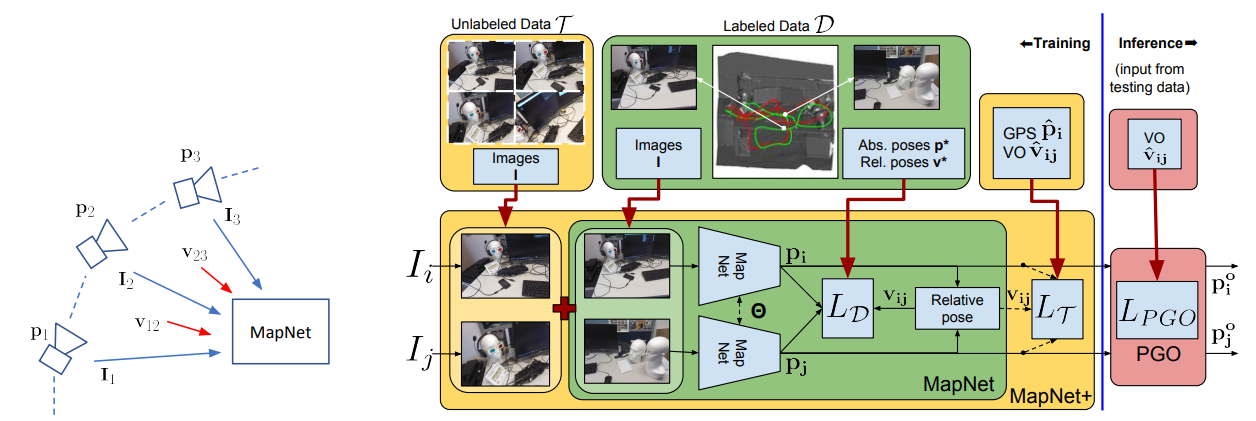
\includegraphics[width=\textwidth]{pics/Chapter2/mapnet.png}
    \caption{Minh họa kiến trúc mô hình MapNet \cite{brahmbhatt2018geometryaware}}
\end{figure}
Năm 2019, tác giả Xue và những cộng sự \cite{xue2019local} cũng có một hướng tiếp cận tương tự khi hồi quy vị trí máy ảnh thông qua những ràng buộc về không gian - thời gian, trong đó đặc trưng cục bộ cải thiện định vị toàn cục - gọi là "Cục bộ hỗ trợ toàn cục" (Local Support Global - LSG). Thêm vào đó, LSG đề xuất sử dụng một đánh giá đã được “tăng cường nội dung” để ước lượng lỗi vị trí và tinh chỉnh dựa trên chuyển động, để tối ưu hóa dự đoán vị trí thông qua các ràng buộc chuyển động. LSG sử dụng một hàm mất mát vị trí toàn cầu $L_g$ lấy từ hồi quy tuyệt đối, hàm mất mát hồi quy đo lường cảm biến trực quan $L_{vo}$, các ràng buộc hình học và hàm mất mát liên kết chuyển động $L_{joint}$ để tối ưu hóa hồi quy vị trí như sau:
\begin{center}
    $l_{total} = l_g + l_{vo} + l_{joint}$
\end{center}
\begin{figure}[H]
    \centering
    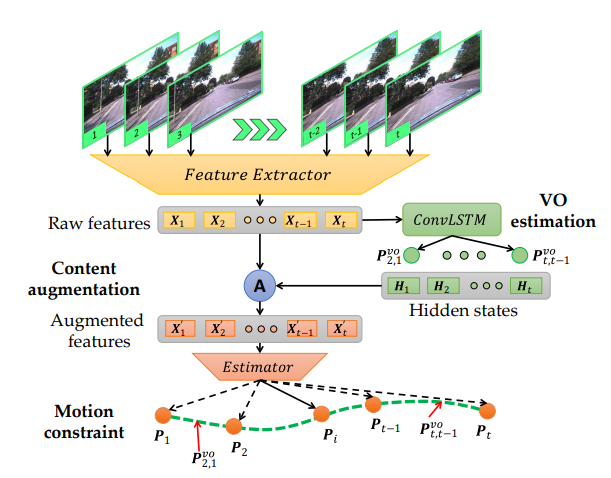
\includegraphics[width=0.8\textwidth]{pics/Chapter2/lsg.png}
    \caption{Minh họa kiến trúc mô hình LSG \cite{xue2019local}}
\end{figure}
\newpage
VlocNet \cite{valada2018deep} cũng học đồng thời đo lường cảm biến trực quan như một tác vụ phụ để hồi quy vị trí toàn cục với hai mạng phụ. Mất mát nhất quán hình học được điều chỉnh để giảm thiểu tối đa lỗi vị trí, được định nghĩa như sau:
\begin{center}
    $l(I_{total}) = (I_{i_x} + I_{ij_x})exp(-\hat{s}_x) + (I_{i_q} + I^{q}_{ij})exp(-\hat{s}_q)+ \hat{s}_q$
\end{center}
\begin{figure}[H]
    \centering
    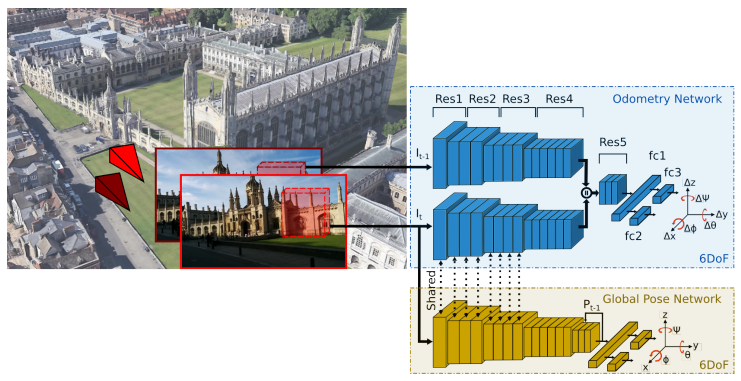
\includegraphics[width=0.9\textwidth]{pics/Chapter2/vlocnet.png}
    \caption{Minh họa kiến trúc mô hình VlocNet \cite{valada2018deep}}
\end{figure}
VlocNet++ \cite{Radwan_2018} giới thiệu kiến thức ngữ nghĩa vào hồi quy vị trí, kết hợp thông tin hình học-thời gian với các đặc trưng ngữ nghĩa cùng một lúc. Hàm mất mát của VlocNet++ kết hợp hồi quy vị trí toàn cục, mất mát đo lường cảm biến trực quan và mất mát Entropy chéo cho mất mát phân đoạn ngữ nghĩa cùng một lúc, với ba yếu tố $\hat{s}_{log}$, $\hat{s}_{vo}$ và $\hat{s}_{seg}$ để cân bằng ba thành phần này:
\begin{center}
    $ l(I_{total}) = l_{loc}exp(-\hat{s}_{loc})+ \hat{s}_{loc}+l_{vo}exp(-\hat{s}_{vo})+ \hat{s}_{vo}+l_{seg}exp(-\hat{s}_{seg})+ \hat{s}_{seg}$
\end{center}
\begin{figure}[H]
    \centering
    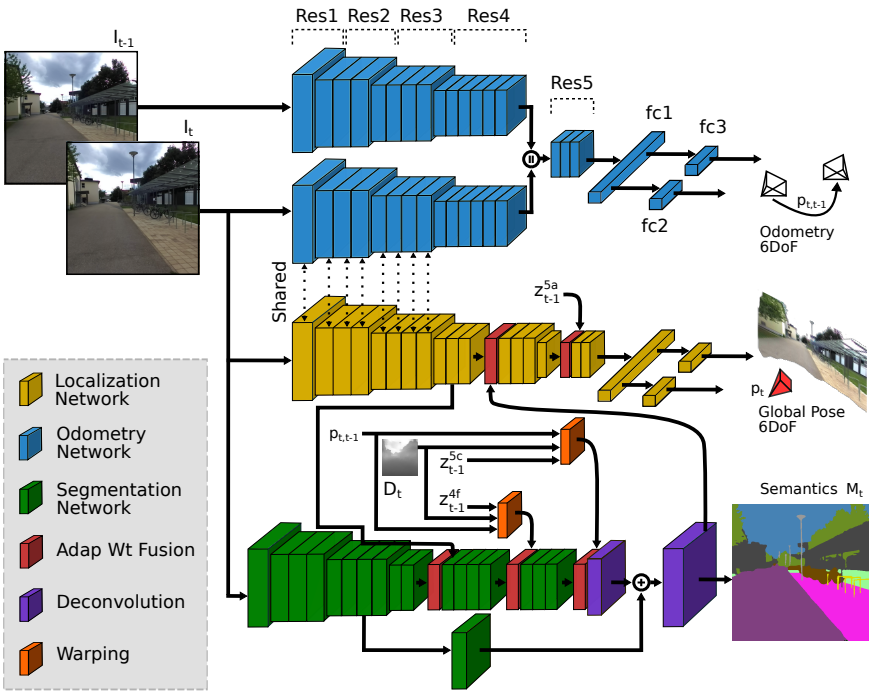
\includegraphics[width=\textwidth]{pics/Chapter2/vlocnetplus.png}
    \caption{Minh họa kiến trúc mô hình VlocNet++ \cite{Radwan_2018}}
\end{figure}
Một bản mở rộng của AtLoc, AtLocPlus \cite{wang2019atloc} cũng kết hợp các ràng buộc thời gian để học cùng lúc mất mát vị trí tuyệt đối và mất mát vị trí tương đối, dẫn đến hiệu suất tốt hơn AtLoc trong việc sử dụng một đầu vào ảnh đơn. AtLocPlus sử dụng hàm mất mát giống với MapNet.

DGRNet \cite{lin2019deep} đề xuất một kiến trúc với một mạng con hồi quy vị trí tương đối RCNN1, một mạng con hồi quy vị trí toàn cục RCNN2 và lớp kết hợp kết nối đầy đủ dùng để trích xuất đặc trưng từ ảnh. Ràng buộc biến đổi chéo (Cross transformation constraint – CTC) và sai số toàn phương trung bình (Mean squared error – MSE) được áp dụng vào hàm mất mát để cải thiện hiệu suất hồi quy. DGRNet đã sử dụng kết hợp hàm mất mát tương đối, toàn cục, CTC $\hat{l}_i$ và sự thật nền tảng $\hat{P}_i$ như sau:
\begin{center}
    $ w = \underset{w}{argmin} \frac{1}{N}^{N}_{i=1} \sum_{k=0}^{6}(l^i_k) + \sum_{j=0}^{4}\left \| P^ij - \hat{P}^i_j \right \|^2_2 $
\end{center}
\begin{figure}[H]
    \centering
    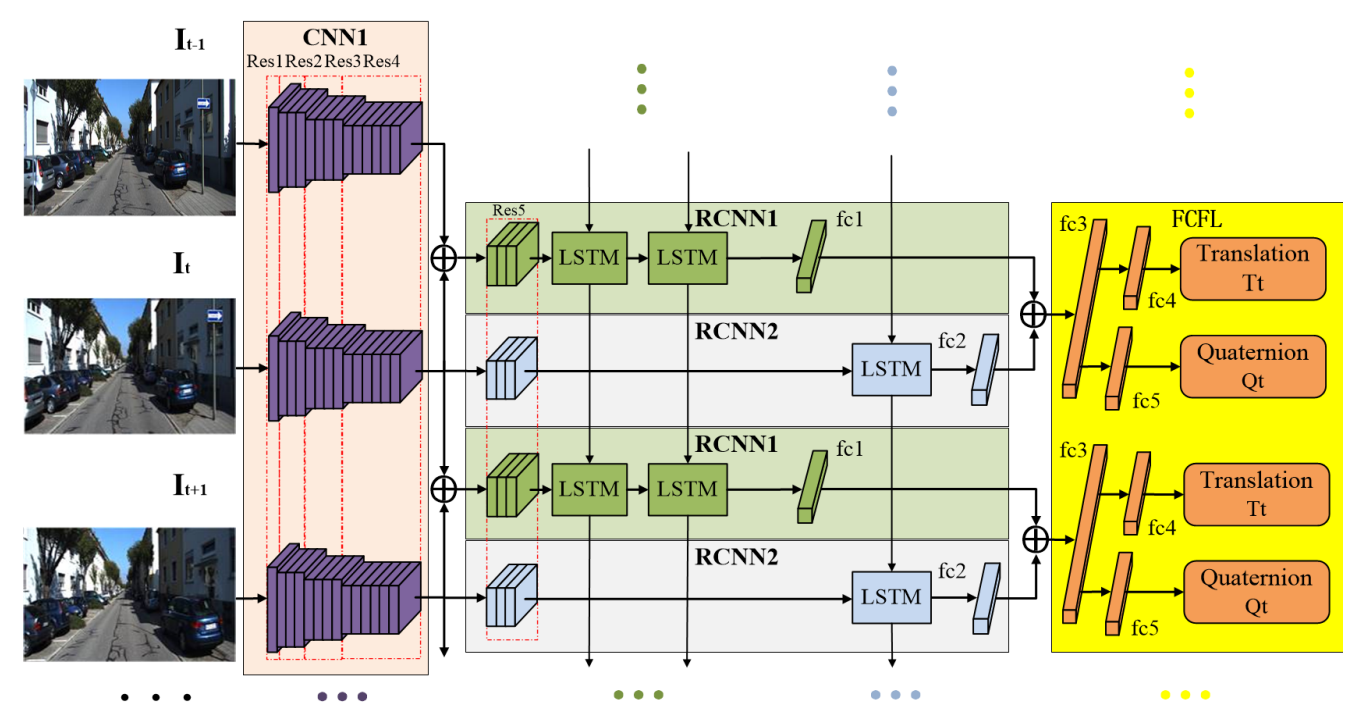
\includegraphics[width=\textwidth]{pics/Chapter2/dgrnet.png}
    \caption{Minh họa kiến trúc mô hình DGRNet \cite{lin2019deep}}
\end{figure}
\subsubsection*{Hồi quy vị trí tuyệt đối qua đoạn phim - Absolute pose regression through video}

Không chỉ đơn ảnh hay đa ảnh, ngay cả đoạn phim cũng có thể được sử dụng để thêm một ràng buộc thời gian có tính trơn tru hơn cho hồi quy vị trí. Các đoạn phim hay các dữ liệu cảm biến khác đều có thể được truy cập dễ dàng bởi các thiết bị di động. Đoạn phim có thể được đồng bộ hóa với các dữ liệu đầu vào khác như đo lường cảm biến trực quan, các cảm biến IMU như đồng hồ tăng tốc và đồng hồ quay và dữ liệu GNSS bằng thông tin thời gian , cụ thể là bằng cách căn chỉnh các mốc thời gian. Với một quy trình tương tự như các phương pháp ARP dựa trên hình ảnh đơn và chuỗi hình ảnh, ARP dựa trên đoạn phim cũng hồi quy độ dời và hướng quay thông qua bộ trích xuất đặc trưng là một mạng nơ-ron tích chập và bộ hồi quy vị trí cục bộ.

VidLoc \cite{clark2017vidloc} đề xuất một mô hình hồi quy vị trí máy ảnh dựa trên việc kết hợp CNN – RNN, mục đích là có thể khiến quá trình dự đoán vị trí từ ảnh hay một đoạn phim được trơn tru hơn. Mạng được xây dựng bằng cách sử dụng GoogLeNet Inception \cite{szegedy2014going} mà không dùng đến lớp kết nối đầy đủ để trích xuất đặc trưng ảnh và một mô-đun LSTM hai chiều để mô hình hóa thông tin thời gian với các ô nhớ.  Hàm mất mát của VidLoc được tính bằng tổng của lỗi vị trí và lỗi hướng quay từ đầu ra của LSTM như sau:
\begin{center}
    $ l = \sum_{t=1}^T \alpha_1 \left \| x_t - \hat{x}_t \right \| + \alpha_2 \left \| q_t - \hat{q}_t \right \| $
\end{center}
Với $[x_t, q_t]$ và $[\hat{x}_t, \hat{q}_t]$ đại diện cho sự thật nền tảng và giá trị dự đoán cho độ dời vị trí và hướng quay.
\begin{figure}[H]
    \centering
    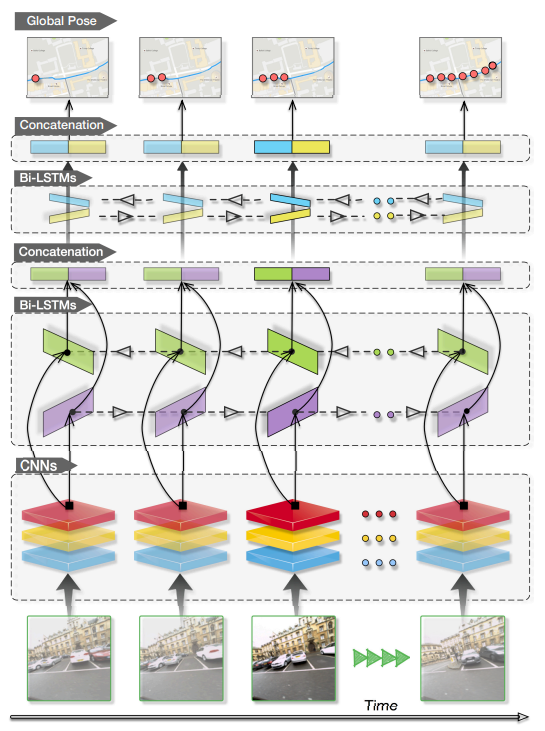
\includegraphics[width=0.9\textwidth]{pics/Chapter2/vidloc.png}
    \caption{Minh họa kiến trúc mô hình VidLoc \cite{clark2017vidloc}}
\end{figure}
\newpage
MapNet+ và MapNet+PGO \cite{brahmbhatt2018geometryaware} mang cùng một kiến trúc mạng với MapNet trích xuất đặc trưng qua mạng ResNet34 và dùng một lớp tổng hợp trung bình toàn cục. Không chỉ dùng mất mát vị trí tuyệt đối, mất mát đo lường cảm biến trực quan cũng được tính toán để cải thiện hiệu suất dự đoán vị trí của MapNet. Phương pháp này cũng đồng thời tích hợp dữ liệu GNSS và IMU để giúp cải thiện hồi quy vị trí. Điều này giúp kết hợp dữ liệu đã được gắn nhãn và dữ liệu chưa gắn nhãn từ VO hay cảm biến để phục vụ cho việc học tự giám sát và đã thể hiện hiệu suất tốt dưới những điều kiện khó khăn, thử thách như thay đổi môi trường ngoài, thiếu sáng,... .
\begin{center}
    $l = l_{labelled data} + l_{unlabelled data}$
\end{center}
Với mất mát từ dữ liệu chưa gắn nhãn có thể được tính toán thông qua việc kết hợp vị trí máy ảnh tương đối $v_ij$ và VO $\hat{v}_ij$ hay các cảm biến khác như IMU và GNSS.

MapNet+PGO đã có thể cải thiện hiệu suất đồng thời giảm thiểu chi phí tính toàn thông qua việc sử dụng cải thiện đồ thị vị trí (PGO) để kết hợp kết quả vị trí MapNet+ và VO.

\subsubsection*{Kết luận}
Xét về các phương pháp mang hướng hồi quy vị trí tuyệt đối thông qua một ảnh duy nhất, các nghiên cứu có xu hướng tiến tới việc hàm mất mát tự động hóa, không sử dụng siêu tham số và mang nhiều thông tin hơn để giảm việc sử dụng các tham số cố định. Khởi đầu từ PoseNet với việc sử dụng một hàm mất mát cố định để tính tổng độ dời và hướng quay sử dụng một số tham số cân bằng. Sau đó, một hàm mất mát có trọng số học được \cite{wang2019atloc, bui2019adversarial} đã được đề xuất bằng cách thêm độ không đảm bảo phương sai đồng nhất để tự động cân bằng mất mát độ dời và hướng quay, tránh sử dụng siêu tham số đồng thời vượt qua hiệu suất của phương pháp sử dụng hàm mất mát cố định. Ngoài phương pháp hàm mất mát cố định và hàm mất mát với trọng số học được, một số công trình \cite{kendall2017geometric, Cai2018AHP} đề xuất sử dụng mất mát lỗi tái chiếu và mất mát GPoseNet để thêm các định dạng thông tin khác như phân phối xác suất của vị trí - hướng quay đầu ra để cải thiện hàm mất mát.

Với việc sử dụng nhiều ảnh cũng như học kết hợp các tác vụ phụ, các mô hình đã có thể không chỉ thu được kết quả định vị mà còn có được thông tin khác như VO, thông tin ngữ nghĩa,etc. MapNet, VlocNet, AtLocPlus \cite{wang2019atloc} kết hợp cả hàm mất mát vị trí tương đối và vị trí tuyệt đối để cải thiện hiệu quả tác vụ hồi quy. LSG \cite{xue2019local} áp dụng một ràng buộc chuyển động vào hàm mất mát trong khi đó VlocNet++ \cite{Radwan_2018} thì đề xuất thêm ràng buộc ngữ nghĩa vào. DGRNet \cite{lin2019deep} kết hợp CTC và MSE vào quá trình tính toán hàm mất mát.

Cho rằng các phương pháp hồi quy vị trí tuyệt đối thông qua ảnh đang bỏ phí giá trị của các ràng buộc thời gian, một số công trình \cite{clark2017vidloc, brahmbhatt2018geometryaware} đề xuất việc tận dụng các đoạn phim làm đầu vào cho tác vụ hồi quy vị trí. VidLoc \cite{clark2017vidloc} sử dụng RNN hai chiều để hồi quy vị trí 6DoF của máy ảnh. MapNet+ và MapNet+PGO \cite{brahmbhatt2018geometryaware} chủ yếu tận dụng VO vào hàm mất mát để tăng cường hiệu quả tác vụ hồi quy.

\subsection{Hồi quy vị trí tương đối - Relative Pose Regression}

Mô hình hồi quy vị trí tuyệt đối học cách ánh xạ các pixel của ảnh sang vị trí của máy ảnh, thường được quyết định bởi hệ trục tọa độ của chính cảnh vật cụ thể mà máy ảnh đang chụp. Khác với hồi quy vị trí tuyệt đối, các phương pháp mang hướng tiếp cận hồi quy vị trí tương đối (Relative Pose Regression) chỉ tính toán vị trí tương đối của ảnh và thường được huấn luyện trên những tập dữ liệu đa cảnh để tăng cường khả năng mở rộng mô hình đầu cuối.
\newpage
\subsubsection*{Hồi quy vị trí tương đối thông qua truy xuất rõ ràng - Relative camera pose regression through explicit retrieval}
Quy trình hồi quy vị trí tương đối của máy ảnh có thể được hiểu như một quy trình bao gồm truy xuất ảnh có độ tương đồng cao nhất trong kho dữ liệu với ảnh nhận đầu vào và sau đó dự đoán vị trí tương đối giữa chúng để lấy được vị trí tuyệt đối của ảnh nhận đầu vào. Cho một ảnh $I_a^c$ được chụp từ máy ảnh $c$, thông qua các phương pháp truy xuất ảnh từ kho dữ liệu, chúng ta có được ảnh có độ tương đồng cao nhất $I_b^c$. Nếu có được vị trí nền tảng $p_b$ của ảnh $I_b^c$ và vị trí tương đối giữa hai ảnh là $p_{a->b}$, vị trí tuyệt đối $p_a$ của ảnh đầu vào $I_a^c$ có thể được xác định bằng các phép biến đổi toán học.

NNnet \cite{laskar2017camera} là công trình đầu tiên đề xuất một phương pháp hồi quy vị trí tương đối dựa trên truy xuất ảnh. Đầu vào của phương pháp này là một ảnh và một kho dữ liệu ảnh có bao gồm vị trí nền tảng. Một tập các cặp ảnh được tận dụng để hồi quy vị trí tương đối thông qua một mạng Siamese với hai nhánh ResNet34 đã được hiệu chỉnh và một hàm mất mát cố định. Ảnh có độ tương đồng gần nhất với ảnh nhận đầu vào có thể được tính toán xác định thông qua bộ trích xuất đặc trưng hình thành bởi nhánh mạng CNN, sau đó vị trí tương đối và vị trí nền tảng của ảnh trích xuất sẽ kết hợp để tính toán xác định vị trí tuyệt đối của ảnh đầu vào.
\begin{figure}[H]
    \centering
    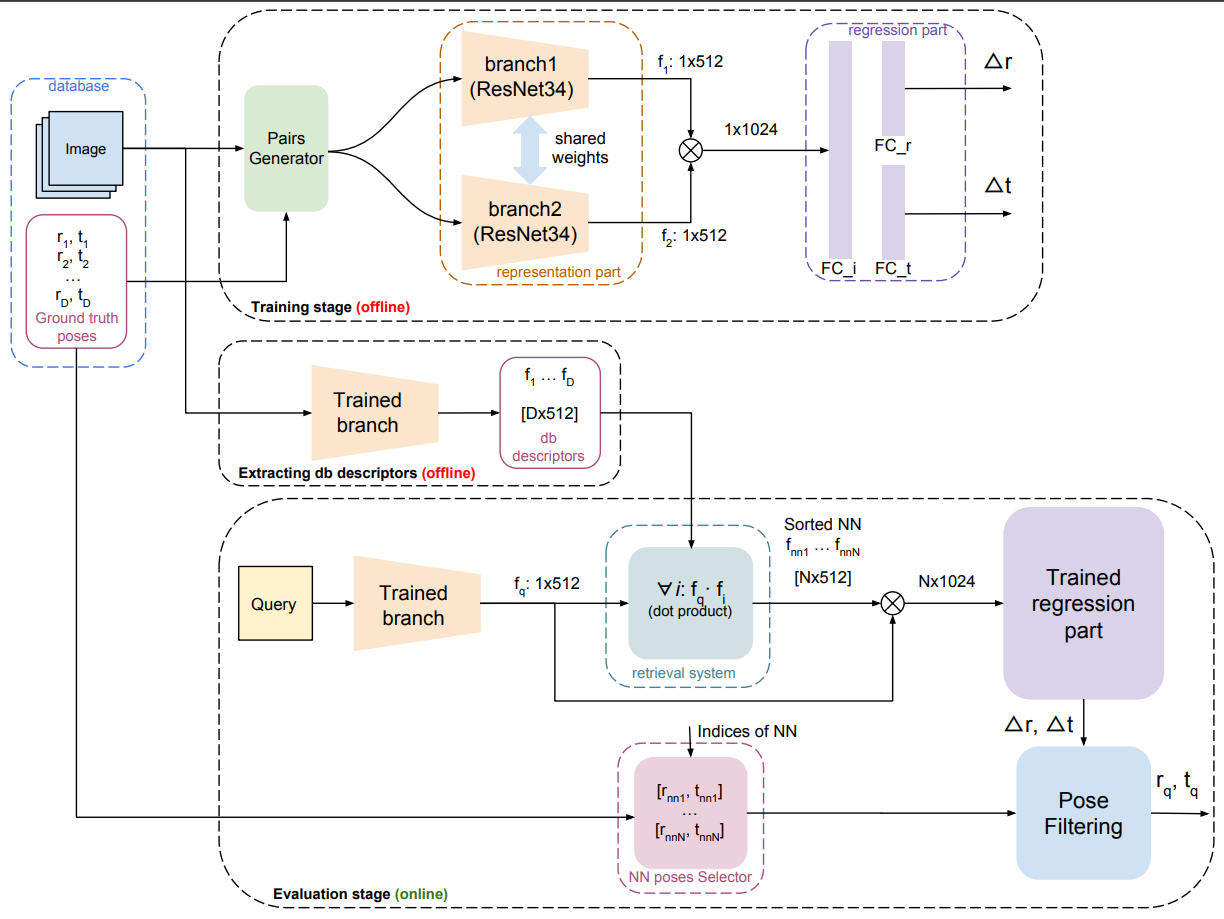
\includegraphics[width=0.9\textwidth]{pics/Chapter2/nnet.png}
    \caption{Minh họa kiến trúc mô hình NNet \cite{laskar2017camera}}
\end{figure}
RelocNet \cite{10.1007/978-3-030-01264-9_46} cải tiến NNet với việc học liên tục thước đo với mục đích học các đặc trưng ảnh toàn cục với một góc nhìn chóp cụt của máy ảnh để cải thiện kết quả, mất mát vị trí tương đối cũng được áp dụng. Mất mát vị trí tương đối học sự khác biệt vị trí giữa hai ma trận vị trí bằng cách sử dụng một biểu diễn ma trận cho hướng quay và độ dời vị trí. Hàm mất mát huấn luyện được định nghĩa như sau:
\begin{center}
    $l = \alpha l_{SE(3)} + \beta l_{frustum}$
\end{center}
\begin{figure}[H]
    \centering
    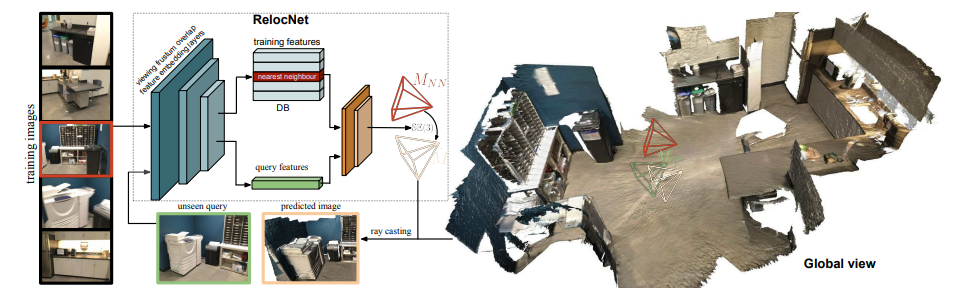
\includegraphics[width=\textwidth]{pics/Chapter2/relocnet.png}
    \caption{Minh họa kiến trúc mô hình RelocNet \cite{10.1007/978-3-030-01264-9_46}}
\end{figure}
Để giải quyết vấn đề hiệu suất giới hạn của các phương pháp hồi quy vị trí tương đối tiền nhiệm do sử dụng cùng đặc trưng cho cả hai bước truy xuất và hồi quy, CamNet \cite{9008579} đề xuất một quy trình chia làm ba bước: truy xuất thô, truy xuất mịn và hồi quy vị trí. Kiến trúc mô hình được xây dựng dựa trên kiến trúc Siamese với ba nhánh mỗi bước. Kiến trúc thô-sang-mịn này đã mang lại những cải tiến về hiệu suất hồi quy cũng như khả năng mở rộng. Hàm mất mát của CamNet lấy ý tưởng dựa trên RelocNet, được định nghĩa như sau:
\begin{center}
    $l = l_{frustum} + l_{angle} + l_{triplet} + l_{PFR} + l_{PRP}$
\end{center}
\begin{figure}[H]
    \centering
    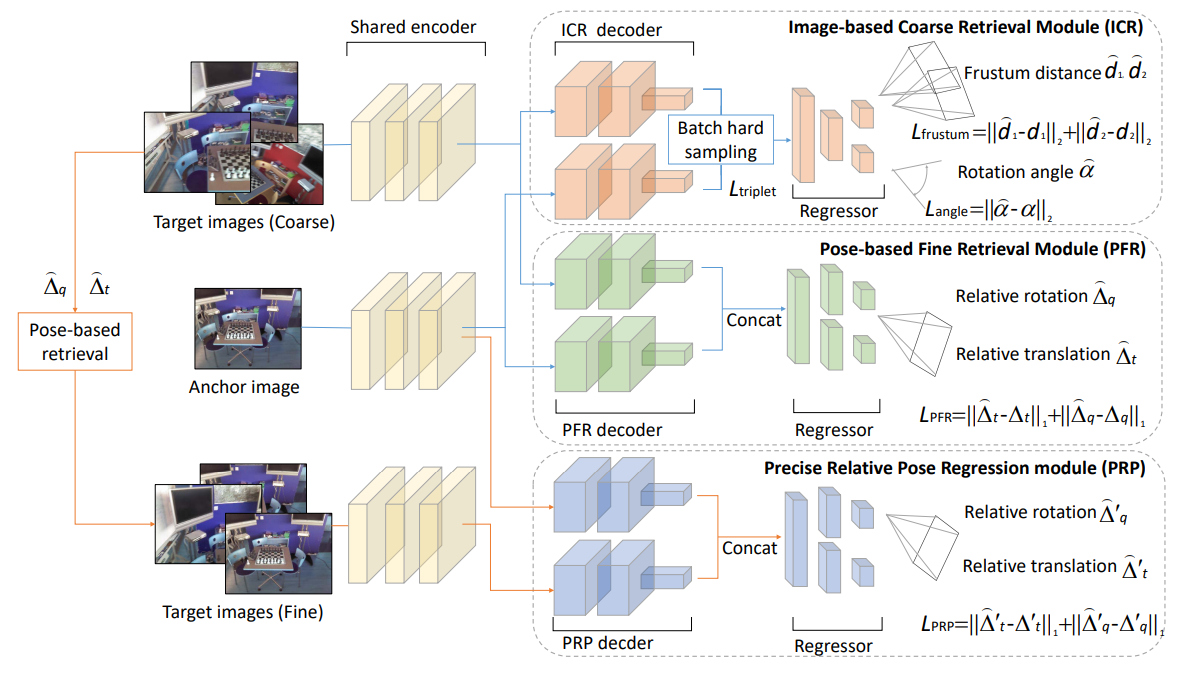
\includegraphics[width=0.9\textwidth]{pics/Chapter2/camnet.png}
    \caption{Minh họa kiến trúc mô hình CamNet \cite{9008579}}
\end{figure}
Qunjie Zhou và những cộng sự \cite{zhou2020learn} sau khi phân tích các phương pháp hồi quy vị trí dựa trên việc truy xuất ảnh đã đề xuất một kiến trúc mới sử dụng ma trận thiết yếu và RANSAC để tính toán vị trí tuyệt đối. Một mạng Siamese ResNet34 với một lớp tìm sự tương ứng cố định (EssNet) và một lớp tìm sự tương ứng đồng thuận lân cận (NC-EssNet) được học để tạo ra một bản đồ điểm tương ứng phục vụ cho mục đích hồi quy về sau của ma trận thiết yếu. Hàm mất mát cải tiến khoảng cách Euclidean giữa ma trận thiết yếu với hai véc-tơ 9 chiều.
\begin{center}
    $l_{ess}(E^*, E) = \left \| e - e^* \right \|_2$
\end{center}
\begin{figure}[H]
    \centering
    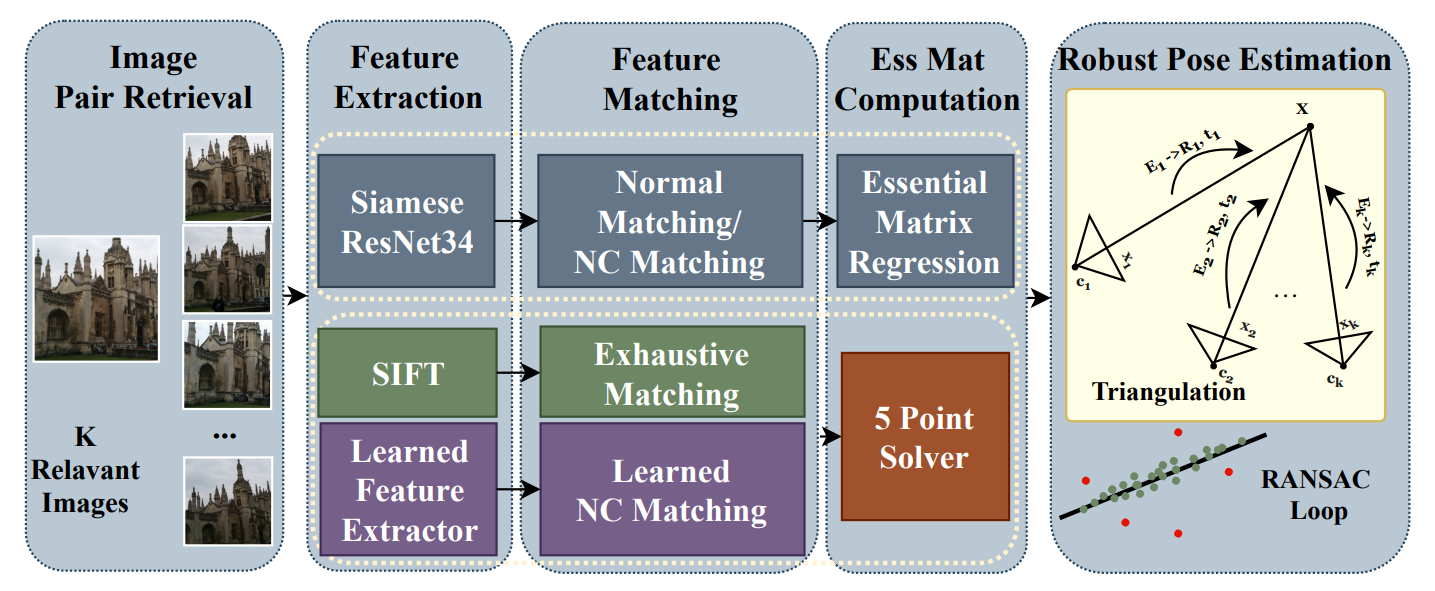
\includegraphics[width=\textwidth]{pics/Chapter2/essnet.png}
    \caption{Minh họa kiến trúc mô hình EssNet \cite{zhou2020learn}}
\end{figure}

\subsubsection*{Hồi quy vị trí tương đối thông qua mạng CNN ngầm - Relative camera pose regression through implicit CNN}
Để tránh việc phải thu thập và xây dựng một kho dữ liệu khổng lồ cũng như tốn kém thời gian thử nghiệm, một số phương pháp tìm cách hồi quy vị trí tương đối của máy ảnh thông qua một mạng Nơ-ron tích chập ngầm.

Relative NN \cite{melekhov2017relative} đề xuất một phương pháp đầu-cuối để hồi quy vị trí tương đối giữa hai máy ảnh bằng hai ảnh đầu vào. Kiến trúc mô hình là một mạng Nơ-ron hỗn hợp Siamese hai nhánh sử dụng mạng AlexNet đã được huấn luyện từ trước được dùng cho việc hồi quy với hàm mất mát Euclidean cố định.
\begin{figure}[H]
    \centering
    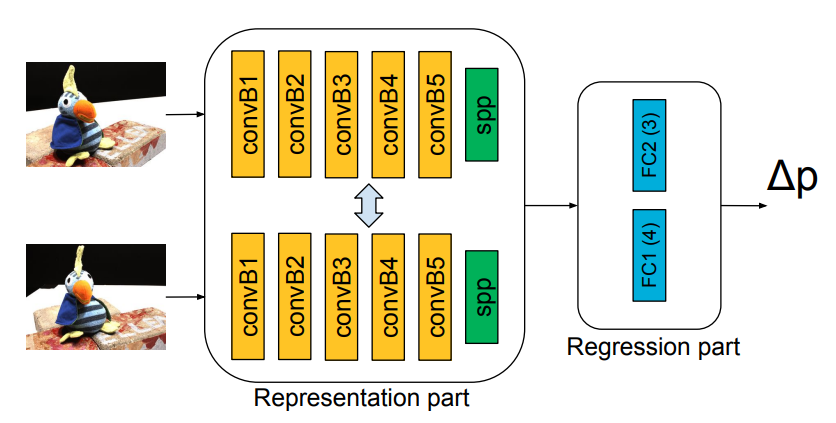
\includegraphics[width=0.9\textwidth]{pics/Chapter2/relativenn.png}
    \caption{Minh họa kiến trúc mô hình Relative Neural Network \cite{melekhov2017relative}}
\end{figure}
AnchorNet \cite{saha2018improved} tìm cách khắc phục vấn đề định vị bằng cách định nghĩa các địa danh thành các điểm mốc để học các điểm mốc tương đối của ảnh đầu vào cũng như độ lệch của chúng. Mô hình đa nhiệm bao gồm việc phân loại hình ảnh truy vấn đầu vào theo các điểm mốc cụ thể và tìm sự chênh lệch so với điểm mốc đã phân loại, điều này dẫn đến việc hình thành hàm mất mát. $\hat{C}$, $X$, và $Y$ đại diện cho kết quả phân loại và sự chênh lệch với sự thật nền tảng.
\begin{center}
    $l = \sum_i[(X_i - \hat{X}_i)^2 + (Y_i - \hat{Y}_i)^2]\hat{C}^i$
\end{center}
\begin{figure}[H]
    \centering
    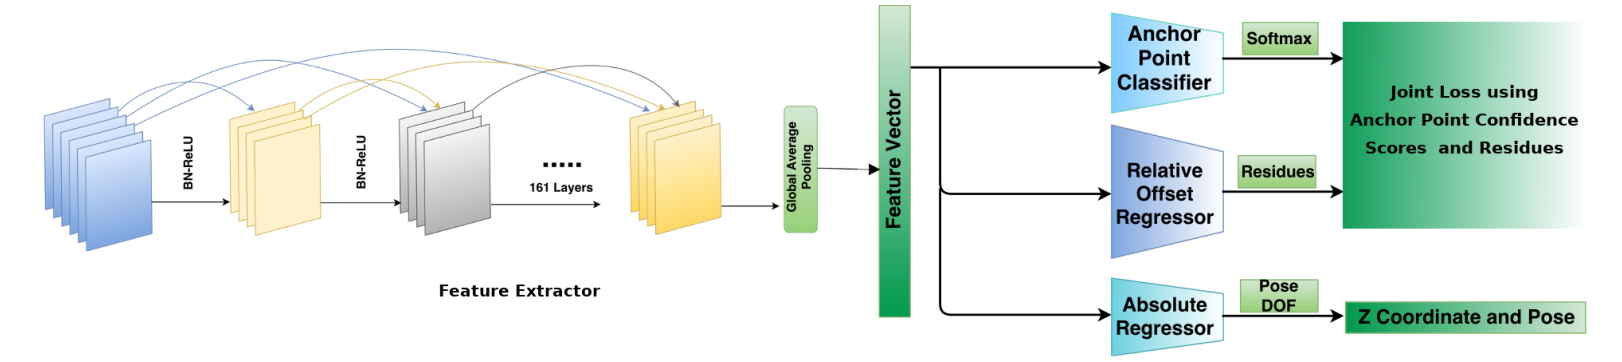
\includegraphics[width=\textwidth]{pics/Chapter2/anchornet.png}
    \caption{Minh họa kiến trúc mô hình AnchorNet \cite{saha2018improved}}
\end{figure}

\subsubsection*{}
Nhận thấy các phương pháp tái định vị trực quan (Visual Relocalization) hiện tại đều cần một kho dữ liệu ảnh khổng lồ nhằm mục đích xây dựng một mô hình 3 chiều cho một khung cảnh nhất định, một nhóm nghiên cứu \cite{arnold2022mapfree} đề xuất phương pháp mang tên "Tái định vị không cần bản đồ (Map-free Relocalization)" với việc chỉ sử dụng duy nhất một ảnh làm đầu vào mà không cần phải xây dựng mô hình 3 chiều cho cảnh. \cite{arnold2022mapfree} đã đề xuất hai phương pháp khác nhau để có thể xác định vị trí, góc quay chính xác từ một ảnh: thứ nhất là tận dụng ma trận thiết yếu kết hợp với các kỹ thuật tìm sự tương ứng giữa đặc trưng ảnh, thứ hai là hồi quy vị trí tương đối.
\begin{figure}[H]
    \centering
    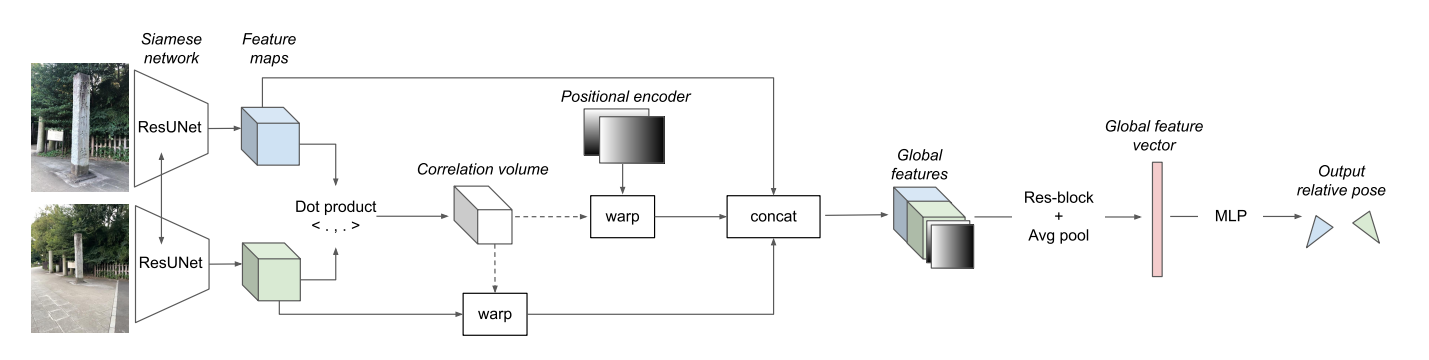
\includegraphics[width=\textwidth]{pics/Chapter2/mapfreeRPR}
    \caption{Minh họa kiến trúc mô hình hồi quy vị trí tương đối của Map-free \cite{arnold2022mapfree}}
\end{figure}

\subsubsection*{Kết luận}
Để thực hiện tác vụ hồi quy vị trí tương đối, các phương pháp dựa trên truy xuất ảnh \cite{laskar2017camera, 10.1007/978-3-030-01264-9_46, 9008579, zhou2020learn} tận dụng một quy trình nhiều bước để lấy được vị trí tuyệt đối với bước truy xuất ảnh làm trọng tâm. NNnet \cite{laskar2017camera} là công trình đầu tiên đề xuất một phương pháp hồi quy vị trí tương đối dựa trên truy xuất ảnh, với RelocNet \cite{10.1007/978-3-030-01264-9_46} tìm cách cải tiến NNet với việc học liên tục thước đo với mục đích học các đặc trưng ảnh toàn cục kết hợp góc nhìn chóp cụt của máy ảnh để cải thiện kết quả. CamNet \cite{9008579} đề xuất một quy trình chia làm ba bước: truy xuất thô, truy xuất mịn và hồi quy vị trí với ba nhánh CNN mỗi bước và đã mang lại những cải tiến về hiệu suất hồi quy cũng như khả năng mở rộng.

Trong khi đó các phương pháp dựa trên CNN \cite{melekhov2017relative, saha2018improved, arnold2022mapfree} lại đề xuất một hướng giải quyết để hồi quy trực tiếp vị trí tương đối ngay trong mạng nơ-ron. Relative NN \cite{melekhov2017relative} đề xuất một mô hình đầu-cuối Siamese hai nhánh để hồi quy vị trí tương đối giữa hai ảnh đầu vào. AnchorNet \cite{saha2018improved} tìm cách khắc phục vấn đề định vị bằng cách định nghĩa các địa danh thành các điểm mốc để học các điểm mốc tương đối của ảnh đầu vào cũng như độ lệch của chúng. Map-free \cite{arnold2022mapfree} đề xuất việc không sử dụng ảnh để tái kiến trúc lại cảnh, đồng thời cung cấp hai phương hướng để hồi quy vị trí từ một ảnh.

\section{Phân tích và tổng hợp}

\subsection*{Nhận dạng địa điểm trực quan}

Nhận xét những kết quả tổng hợp được từ các bài báo khoa học từ những ngày đầu phát triển của bài toán nhận dạng địa điểm trực quan, có thể thấy, bài toán đã được đặt trong giới hạn dữ liệu (dữ liệu ảnh RGB thuần, không có độ sâu D) mang tính chất quyết định đến khả năng xây dựng, phát triển và duy trì hoạt động của các mô hình trước phạm vi dữ liệu lớn về không gian, thời gian và các miền khác. Tất cả các nỗ lực nghiên cứu đến nay đều đang hướng đến việc gia tăng hiệu năng của các mô hình để cạnh tranh với các mô hình không chịu giới hạn. Xét những mô hình đạt hiệu năng cao nhất trong thời điểm hiện tại, có thể thấy, tuy các mô hình trong giới hạn vẫn chưa vượt qua được các mô hình này, phạm vi dữ liệu của chúng đã được mở rộng hơn một cách đáng kể trong khi tác động đến tài nguyên phát triển và duy trì thấp. Đây là một điểm mạnh nổi bật, cho phép các mô hình có thể được áp dụng rộng rãi, nhanh chóng và dễ dàng duy trì trong thực tế. Vì lý do này, chúng tôi cho rằng các mô hình giải quyết bài toán nhận dạng địa điểm trực quan trong giới hạn dữ liệu trên vẫn là một hướng đi phù hợp và có tiềm năng để hoàn thành mục tiêu đề ra cho báo cáo. Bằng cách cải tiến cấu trúc tập trung bằng cấu trúc trộn đặc trưng, hiệu năng của mô hình tổng hợp đặc trưng biểu diễn MixVPR \cite{alibey2023mixvpr} đạt được kết quả cạnh tranh so với các mô hình có hiệu quả cao nhất hiện tại. Sau khi phân tích và so sánh, chúng tôi tin rằng, mô hình MixVPR có tiềm năng phát triển cao và phù hợp để áp dụng cho bài toán định vị trực quan đã đề ra.

\subsection*{Hồi quy vị trí}

Nếu xem xét bài toán định vị trực quan dưới góc nhìn là quy trình hai bước: từ ảnh truy vấn, tìm ảnh truy xuất gần nhất và từ cặp ảnh này, tìm tư thế, vị trí của thiết bị chụp ảnh truy vấn, hiệu năng của bước thứ hai phụ thuộc vào khả năng khai thác các đặc trưng tương quan về góc chụp và thông số thiết bị. Vì các mô hình hồi quy vị trí tuyệt đối thường xuyên gặp vấn đề quá khớp, thiếu tính khái quát, chúng tôi hướng sự tập trung của mình đến các mô hình hồi quy vị trí tương đối. Các mô hình hồi quy vị trí tương đối gần đây tập trung vào mục tiêu tạo mối quan hệ 2D-3D cho các đặc trưng truy xuất được, đòi hỏi sự hiện diện của thông tin độ sâu trong cơ sở dữ liệu truy xuất. Một số bài toán đã tiếp cận vấn đề này bằng cách sử dụng một mô hình khai thác thông tin cấu trúc từ chuỗi hình ảnh (Structure from Motion - SfM), đề xuất thêm một bước tiền xử lý cho quá trình thu thập dữ liệu ảnh RGB. Có thể dễ dàng nhận thấy, với cơ sở dữ liệu tăng dần theo thời gian, khi mô hình được áp dụng và phát triển trên phạm vi lớn, tác động của quá trình SfM sẽ nhanh chóng vượt ngoài kiểm soát. Để giảm thiểu tác động đến tài nguyên, có thể thấy một mô hình lý tưởng cần có khả năng truy xuất và khai thác được đặc trưng tương quan của một cặp ảnh, tính toán được tư thế và vị trí chính xác của một ảnh khi có được tư thế và vị trí ảnh còn lại mà không phải mã hóa hay tổng hợp thêm đặc trưng vào cơ sở dữ liệu đã có. Vì thế, khả năng tạo mối quan hệ 2D-2D sẽ là yếu tố quyết định dẫn đến thành công cho mô hình.

Nhận thấy mô hình Map-free \cite{arnold2022mapfree} đề xuất nhiều hướng tiếp cận cho bài toán: 3D-3D (sử dụng quy trình Procrustes), 2D-3D (sử dụng thuật toán Perspective-n-Point) và 2D-2D (sử dụng ma trận thiết yếu và khai thác độ sâu), chúng tôi đã tìm hiểu về quy trình này. Quy trình tính toán tương quan 2D-2D mà bài nghiên cứu để xuất truyền đặc trưng trích xuất được từ một mô hình trích xuất đặc trưng tương quan đã được huấn luyện sẵn vào một thuật toán tìm ma trận thiết yếu và khai thác tỷ lệ độ sâu. Khi cân nhắc hiệu suất cao của quá trình tính toán vị trí tương đối dựa vào ma trận thiết yếu so với quá trình hồi quy trực tiếp \cite{sattler2019understanding}, có thể thấy được tiềm năng phát triển mới cho bài toán định vị trực quan. Đồng thời, quy trình khai thác ma trận thiết yếu có thể được hiện thực thông qua thuật toán giải 5-điểm (5-Point Solver) \cite{nister2004efficient}, giải pháp này cũng gỡ bỏ một phần gánh nặng của quá trình huấn luyện. Sau khi phân tích, chúng tôi tin rằng, mô hình Map-free có tiềm năng hỗ trợ tốt quá trình định vị trực quan của bài toán mà không tác động nhiều đến tài nguyên phát triển và duy trì của mô hình.
